\documentclass[12pt,a4j]{jarticle}
%---------------------------------------------------
\usepackage[dvipdfmx]{graphicx}
\usepackage{amssymb}
\usepackage{amsmath}
\usepackage{ascmac}
\usepackage{setspace}
\usepackage{float}
\usepackage[dvipdfmx,usenames]{color}
\usepackage{colortbl}
\usepackage{algorithm}
\usepackage{algorithmic}
\usepackage{setspace}
\usepackage{udline}
%---------------------------------------------------
\makeatletter
\def\@maketitle{%
\begin{center}%
\let\footnote\thanks
\vspace*{80mm} % この量でタイトルの位置が下がる。
{\LARGE \@title \par}%
\vskip 1.5em%
{\large
\lineskip .5em%
\begin{tabular}[t]{c}%
\@author
\end{tabular}\par}%
\vskip 1em%
{\large \@date}%
\end{center}%
\par\vskip 1.5em}
\makeatother

\title{\Huge 授業支援システム\\外部設計書}
\date{\today}
\author{\large Outing Corporation}
\begin{document}

\maketitle

\newpage

\pagenumbering{arabic}
\newpage
\section{業務の流れ}
% ここから本文を書いてください.
本システムは主に学生の進捗状況並びに質問を整理することで管理者である教師の方々が円滑に授業を行うための、教務支援システムである。

管理者はシステムが内蔵してあるラズベリーパイを、管理者用PCに接続することで利用可能となる。
学生側はラズベリーパイからのWi-Fiをスマートフォンか別のラズベリーパイで受信することによりログインする。
主に管理者は授業に合わせて学生側に映し出す画面を作成することによって、学生ごとに課題をどの程度進めているのかを確認できる。
これは学生側から講義中に行なっている課題の進捗状況をリアルタイムで送信することで実現する。
また学生側は、講義内容や課題に対しての質問を送信する。
この入力された質問は管理者の画面上でどの学生による質問であるのかが表示される。
その場で回答を行なった場合でも、このシステムに書き込んだ場合でも質問自体は授業中であれば学生側も閲覧可能となっている。
この質問と、回答についてはDB(データベース)に蓄積されることにより、翌年度以降の講義改善に役立てることができる。
DBに蓄積されるデータは実際に利用された画面などのデータも格納しているため、一度設定を行うことで次回以降も利用可能になっている。

\newpage
\section{画面遷移図}
% ここから本文を書いてください.
\newpage
\section{各画面の説明}
\subsection{ログイン画面}
\subsubsection{画面の概要}
% 画面の概要
この画面は、システムを利用する管理者および学生がログインするためのものです。
図\ref{fig:01}にイメージ図を示します。

\subsubsection{操作説明}
% 操作説明
ログインする場合は、ユーザIDとパスワードを入力し、「ログイン」ボタンを押します。
ログインが成功すると、管理者アカウントの場合は「管理者用ホーム画面」に遷移し、
学生アカウントの場合は「学生用ホーム画面」に遷移します。
また、登録されていないユーザIDまたはパスワードを入力すると、エラーが表示されます。

アカウントを新規登録する場合は、「新規登録」ボタンを押して「アカウント新規登録画面」に遷移します。

\newpage

% \begin{figure}[phtbp]
  % \begin{center}
    % 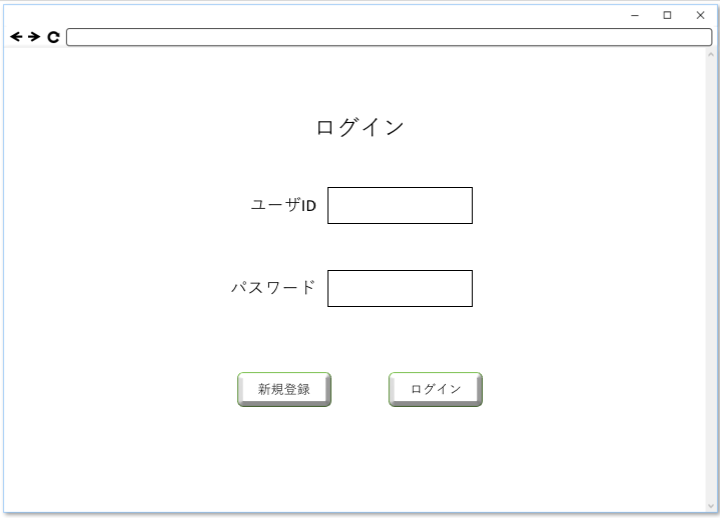
\includegraphics[width=0.6\linewidth,clip]{./img/01.png}
    % \caption{ログイン画面のイメージ図}\label{fig:01}
  % \end{center}
% \end{figure}

% \begin{figure}[phtbp]
  % \begin{center}
    % 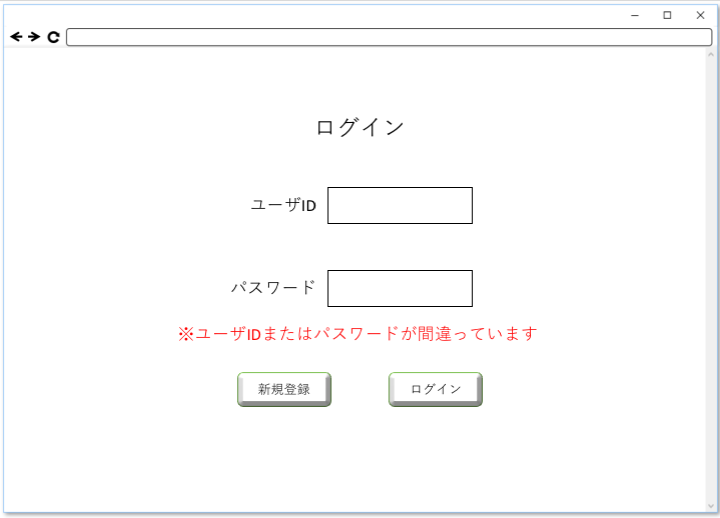
\includegraphics[width=0.6\linewidth,clip]{./img/02.png}
    % \caption{ログイン画面のエラー表示イメージ図}\label{fig:02}
  % \end{center}
% \end{figure}

\begin{figure}[htbp]
 \begin{minipage}{0.5\hsize}
  \begin{center}
   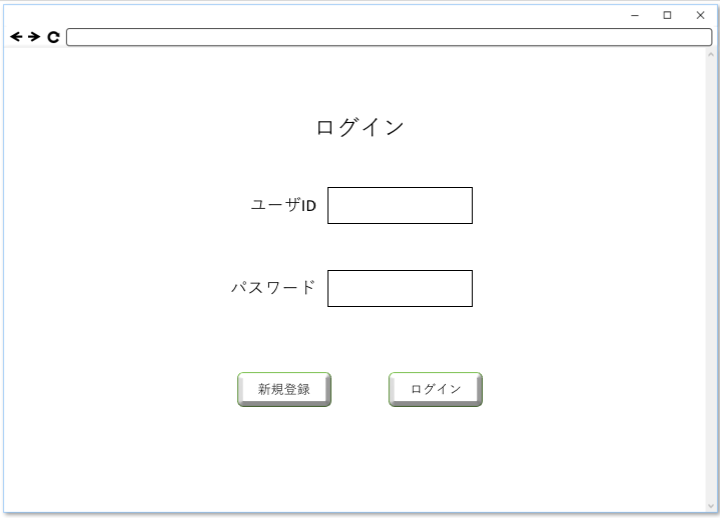
\includegraphics[width=1\linewidth,clip]{./img/01.png}
  \end{center}

 \end{minipage}
 \begin{minipage}{0.5\hsize}
  \begin{center}
   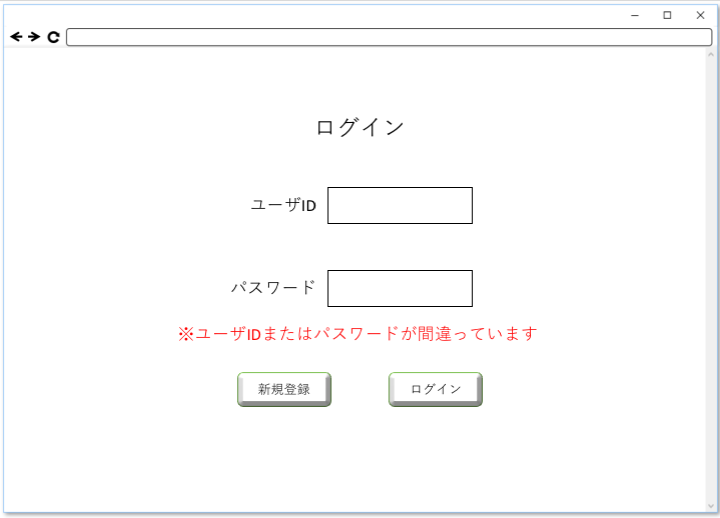
\includegraphics[width=1\linewidth,clip]{./img/02.png}
  \end{center}
  %\caption{ログイン画面のエラー表示イメージ図}\label{fig:02}
 \end{minipage}
 \caption{ログイン画面のイメージ図(左:通常時、右:エラー発生時)}\label{fig:01}
\end{figure}

\subsection{アカウント新規登録画面\label{creat_account}}
\subsubsection{画面の概要}
% 画面の概要
この画面は、学生がアカウントを新規登録するためのものです。
図\ref{fig:03}にイメージ図を示します。

\subsubsection{操作説明}
% 操作説明
ユーザID、氏名(フルネーム)およびパスワードを入力します。
なお、パスワードは確認のために2回入力します。
「登録」ボタンを押すとアカウントが登録され、「ログイン画面」に遷移します。

\begin{figure}[htbp]
  \begin{center}
    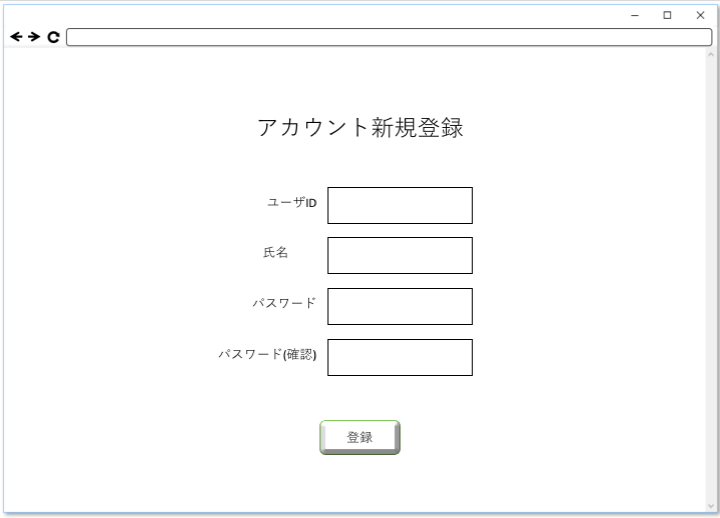
\includegraphics[width=0.5\linewidth,clip]{./img/03.png}
    \caption{アカウント新規登録画面のイメージ図}\label{fig:03}
  \end{center}
\end{figure}

\newpage

\subsection{管理者用ホーム画面}
\subsubsection{画面の概要}
% 画面の概要
この画面は、管理者がログインした際に表示されるものです。
図\ref{fig:04}にイメージ図を示します。

また、全ての管理者用・学生用画面には、この図の右上にある「◯◯がログイン中」というものが表示されます。
この「〇〇」には、ログインしたユーザの氏名が表示されます。
逆三角マーク押すと、図\ref{fig:05}のようなものが表示され、
アカウントの登録情報を変更する画面への遷移やログアウトができるようになっています。

\subsubsection{操作説明}
% 操作説明
「授業選択・作成」ボタンを押すと、「授業選択画面」に遷移します。
また、画面左の最近開いた授業の欄には、最近編集または使用した授業へのリンクが最大6つ表示されます。
このリンクをクリックすると、その授業における「授業回選択画面」に遷移します。

「アカウント新規登録」ボタンを押すと、他の管理者や学生のアカウントを登録する「他のアカウント新規登録画面」に遷移します。

右上の逆三角マークを押し、図\ref{fig:05}のように表示された後、
「登録情報編集」ボタンを押すと、「登録情報編集画面」に遷移します。
また、「ログアウト」ボタンを押すと、ログアウトして「ログイン画面」に遷移します。



\begin{figure}[phtbp]
  \begin{center}
    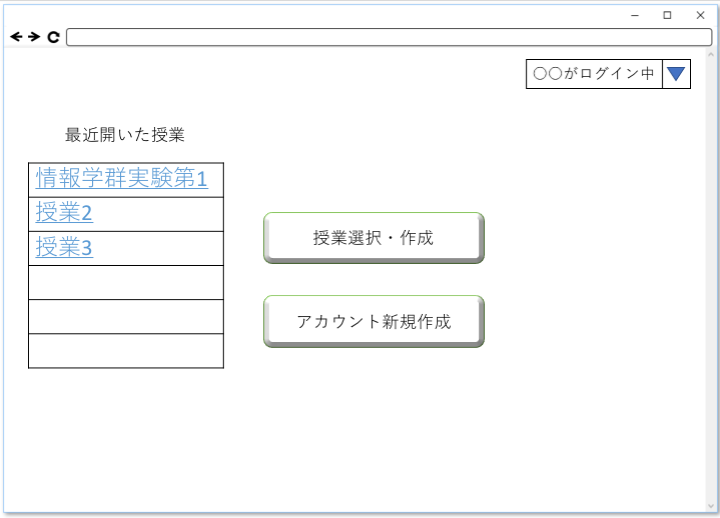
\includegraphics[width=0.8\linewidth,clip]{./img/04.png}
    \caption{管理者用ホーム画面のイメージ図}\label{fig:04}
  \end{center}
\end{figure}

\begin{figure}[phtbp]
  \begin{center}
    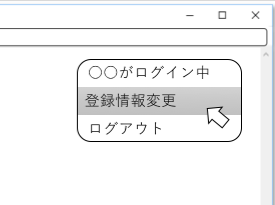
\includegraphics[width=0.2\linewidth,clip]{./img/05_.png}
    \caption{画面右上の逆三角マークを押したときのイメージ図}\label{fig:05}
  \end{center}
\end{figure}

% \begin{figure}[htbp]
 % \begin{minipage}{0.5\hsize}
  % \begin{center}
   % 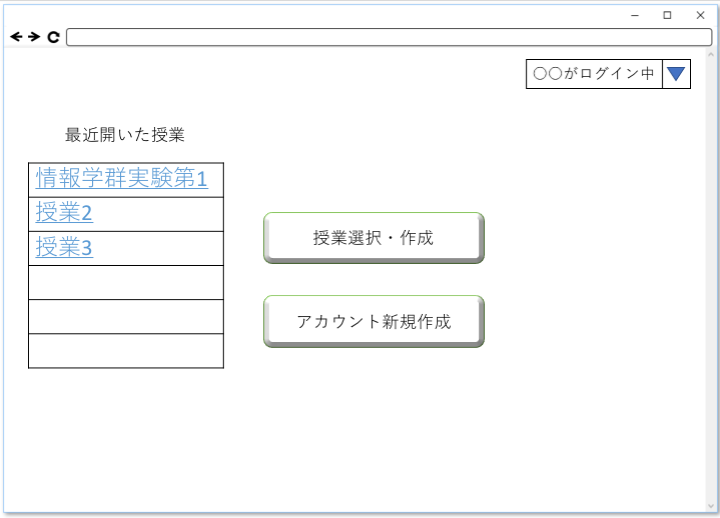
\includegraphics[width=1\linewidth,clip]{./img/04.png}
  % \end{center}
 % \end{minipage}
 % \begin{minipage}{0.5\hsize}
  % \begin{center}
   % 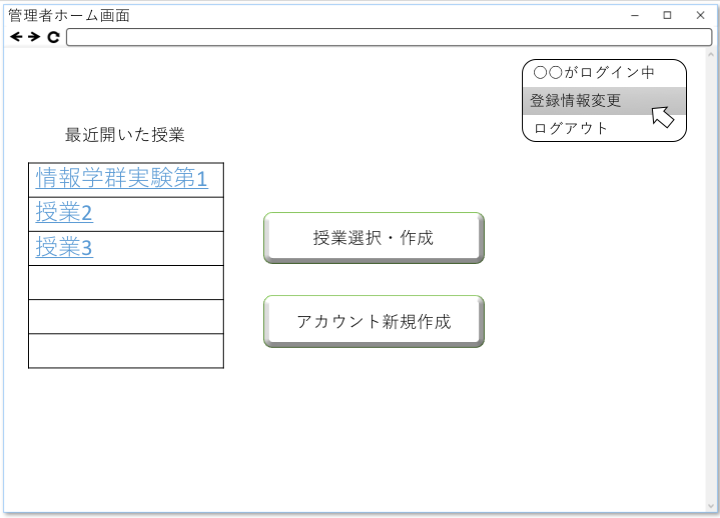
\includegraphics[width=1\linewidth,clip]{./img/05.png}
  % \end{center}
  %\caption{画面右上選択のイメージ図   }\label{fig:05}
 % \end{minipage}
 % \caption{管理者用ホーム画面のイメージ図}\label{fig:04}
% \end{figure}

\newpage

\subsection{登録情報編集画面}
\subsubsection{画面の概要}
% 画面の概要
この画面は、ユーザの登録したユーザIDやパスワードなどの登録情報を編集するためのものです。
図\ref{fig:06}にイメージ図を示します。

\subsubsection{操作説明}
% 操作説明
旧パスワードの欄に現在使用しているパスワード、新パスワードの欄に新しく設定したいパスワードを入力します。
なお、新パスワードは確認のために2回入力します。
「変更」ボタンを押すことで、編集内容が保存されて「管理者ホーム画面」に遷移します。

\begin{figure}[htbp]
  \begin{center}
    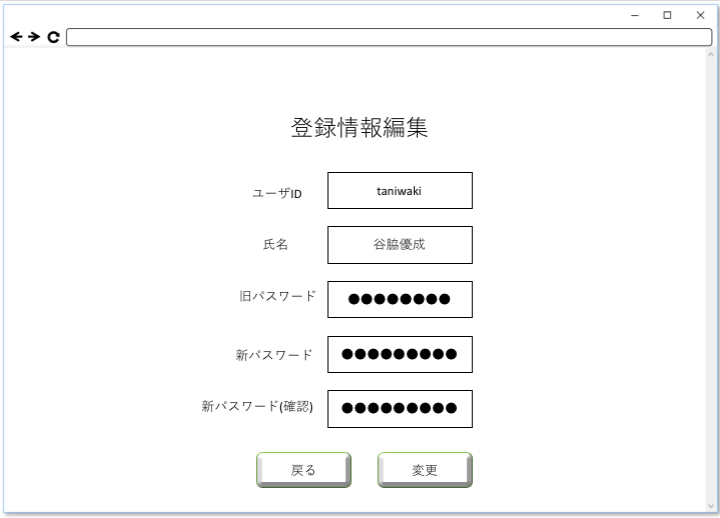
\includegraphics[width=0.8\linewidth,clip]{./img/06.png}
    \caption{登録情報編集画面のイメージ図}\label{fig:06}
  \end{center}
\end{figure}

\newpage

\subsection{他のアカウント新規登録画面}
\subsubsection{画面の概要}
% 画面の概要
この画面は、管理者側が自分以外のアカウントを新規登録するための画面です。
ここでは、新規登録するアカウントの権限レベルを、
「教員」、「アシスタント」、「学生」の中から指定することができ、
主に、新しく教員や授業のアシスタントを登録するときなどに利用します。
図\ref{fig:07}にイメージ図を示します。

\subsubsection{操作説明}
% 操作説明
基本的には、\ref{creat_account}節で述べた、「アカウント新規登録画面」と同じような操作になります。

権限レベルの欄にある逆三角マークを押すことで、図\ref{fig:08}のようなものが表示されます。
「教員」、「アシスタント」、「学生」のいずれかを選択することで、権限レベルを指定することができます。
アカウント登録後は、実際にそのアカウントを使用する人に、パスワードの変更を行っていただきます。

\begin{figure}[phtbp]
  \begin{center}
    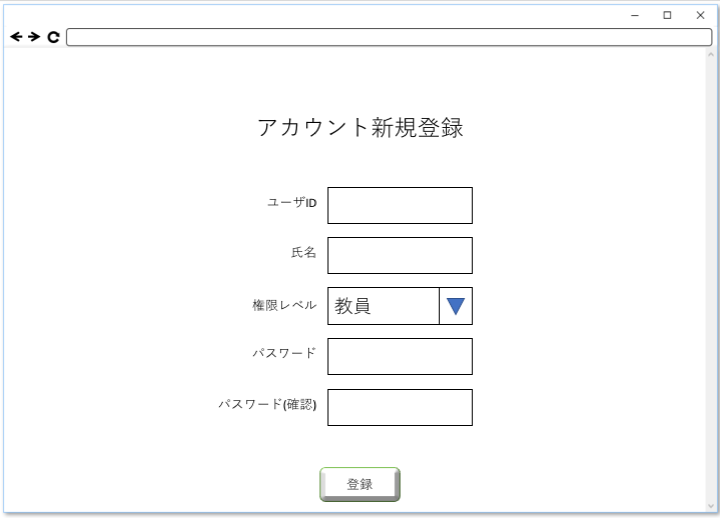
\includegraphics[width=0.8\linewidth,clip]{./img/07.png}
    \caption{管理者用の他のアカウント新規登録画面のイメージ図}\label{fig:07}
  \end{center}
\end{figure}

\begin{figure}[phtbp]
  \begin{center}
    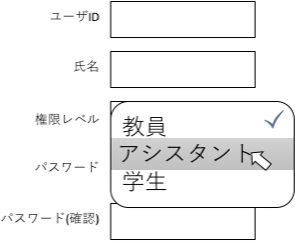
\includegraphics[width=0.35\linewidth,clip]{./img/08_.png}
    \caption{権限レベル選択のイメージ図}\label{fig:08}
  \end{center}
\end{figure}

% \begin{figure}[htbp]
 % \begin{minipage}{0.5\hsize}
  % \begin{center}
   % 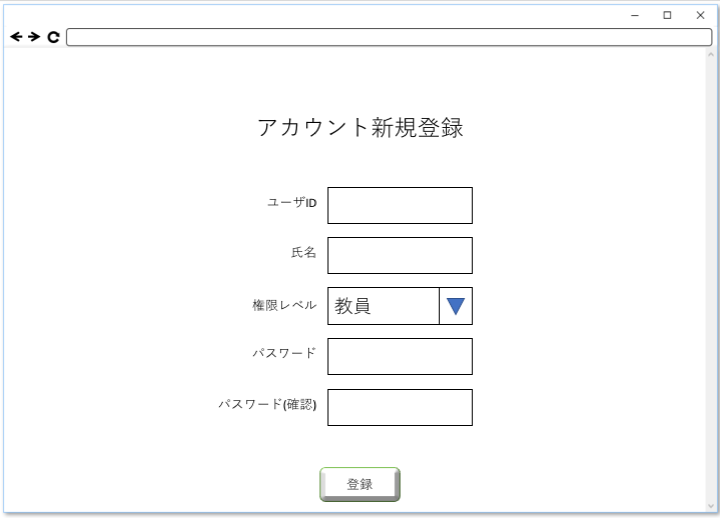
\includegraphics[width=1\linewidth,clip]{./img/07.png}
  % \end{center}
 % \end{minipage}
 % \begin{minipage}{0.5\hsize}
  % \begin{center}
   % 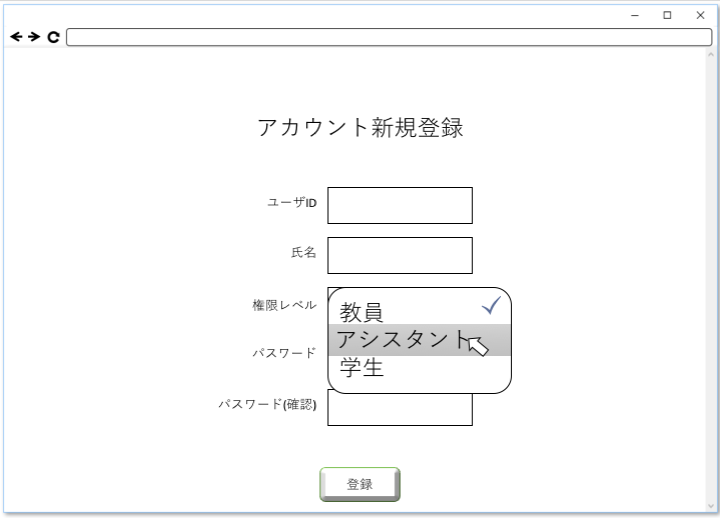
\includegraphics[width=1\linewidth,clip]{./img/08.png}
  % \end{center}
  %\caption{権限レベル選択のイメージ図           }\label{fig:08}
 % \end{minipage}
 % \caption{管理者用の他のアカウント新規登録画面のイメージ図}\label{fig:07}
% \end{figure}

\newpage

\subsection{授業選択画面}
\subsubsection{画面の概要}
% 画面の概要
この画面は、授業の開講、質問の閲覧・編集、グループの編集などを行うときに対象となる授業を選択するためのものです。
また、この画面から、授業の新規作成を行う画面や、すでに作成している授業の編集を行う画面に遷移できます。
図\ref{fig:09}にイメージ図を示します。

\subsubsection{操作説明}
% 操作説明
管理者が作成した授業のリンクが表示されており、そのリンクをクリックすることでその授業の「管理者用の授業回選択画面」に遷移します。
新しい授業を作成したい場合は、「授業新規作成」ボタンを押すことで、「授業新規作成画面」に遷移します。
また、すでに作成している授業の情報を編集したい場合、授業名の横の「編集」ボタンを押すことで、「詳細設定画面2」に遷移します。

\begin{figure}[htbp]
  \begin{center}
    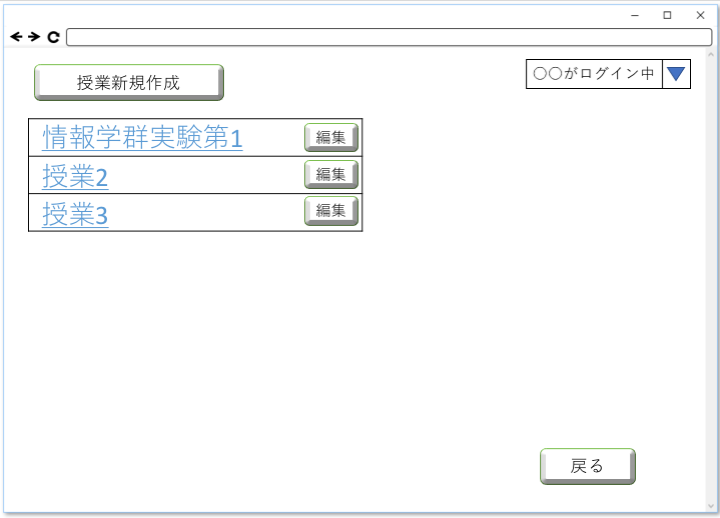
\includegraphics[width=0.7\linewidth,clip]{./img/09.png}
    \caption{授業選択画面のイメージ図}\label{fig:09}
  \end{center}
\end{figure}

\newpage

\subsection{授業新規作成画面}
\subsubsection{画面の概要}
% 画面の概要
この画面は、新しく授業を作成する時の、初期設定を行う画面です。
授業名、個人ワークかグループワーク、質問機能+進捗機能か質問機能のみ、の3つを決めることができます。
図\ref{fig:10}にイメージ図を示します。

\subsubsection{操作説明}
% 操作説明
まず、授業名を入力します。
その後、グループワークなのか、個人ワークなのかを選択し、最後に使用する機能が質問機能と進捗機能なのか、それとも質問機能だけなのかを選択し、「決定」ボタンを押すことで、「詳細設定画面」に遷移します。

\begin{figure}[htbp]
  \begin{center}
    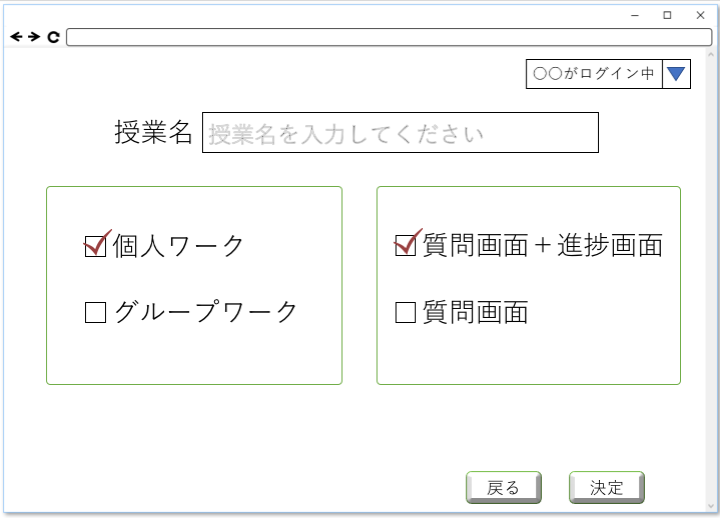
\includegraphics[width=0.7\linewidth,clip]{./img/10.png}
    \caption{授業新規作成画面のイメージ図}\label{fig:10}
  \end{center}
\end{figure}

\newpage

\subsection{詳細設定画面1}
\subsubsection{画面の概要}
% 画面の概要
この画面は、授業回ごとの授業タイトルや課題数を設定する画面です。
また、作成、編集している授業をグループワークで行う場合に、グループの編集が行える画面に遷移できる画面でもあります。
この遷移は「詳細設定画面2」や「詳細設定画面3」でも行えます。
図\ref{fig:11}にイメージ図を示します。

\subsubsection{操作説明}
% 操作説明
授業タイトルには学生側が過去の質問を見ようとした時でもわかるようなタイトルを入力し、課題数にはその回に出る課題の数を入力します。
授業回数を増やしたい場合は、「授業を追加する」ボタンを押すことで、その回の入力欄が追加されていきます。
全ての入力が終われば、「決定」ボタンを押すことで入力内容が保存され、「詳細設定画面2」に遷移します。
また、「グループ編集」ボタンを押すことで、「グループ編集選択画面」に遷移できます。

\begin{figure}[htbp]
  \begin{center}
    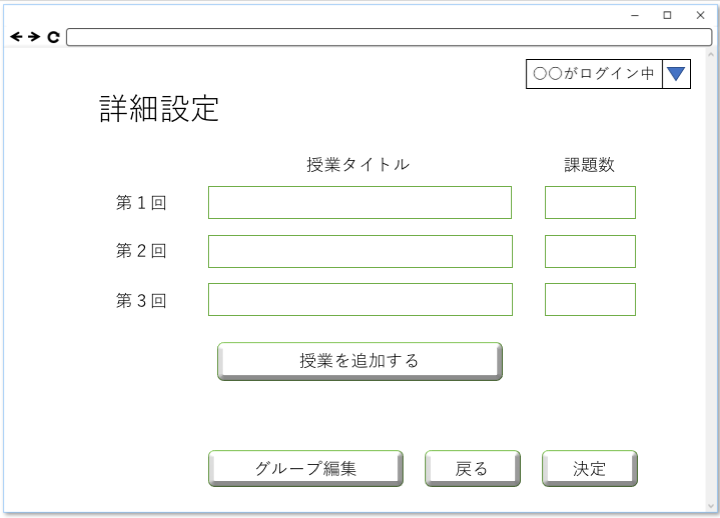
\includegraphics[width=0.7\linewidth,clip]{./img/11.png}
    \caption{詳細設定画面1のイメージ図}\label{fig:11}
  \end{center}
\end{figure}

\newpage

\subsection{詳細設定画面2}
\subsubsection{画面の概要}
% 画面の概要
この画面は「詳細設定画面1」で入力したタイトルとその課題数に応じて課題の内容を入力できる画面に遷移できる画面です。
図\ref{fig:12}にイメージ図を示します。

\subsubsection{操作説明}
% 操作説明
授業タイトルのボタンを押すことでその回の課題内容を入力する「詳細設定画面3」に遷移します。
「詳細設定画面3」に全ての回に応じた課題内容を入力し終わったら、「決定」ボタンを押すことで授業ページが作成されます。
授業タイトルや課題数を編集したり、授業回を新しく追加したい場合は、「授業の追加・編集」ボタンを押すことで「詳細設定画面1」に遷移できます。

\begin{figure}[htbp]
  \begin{center}
    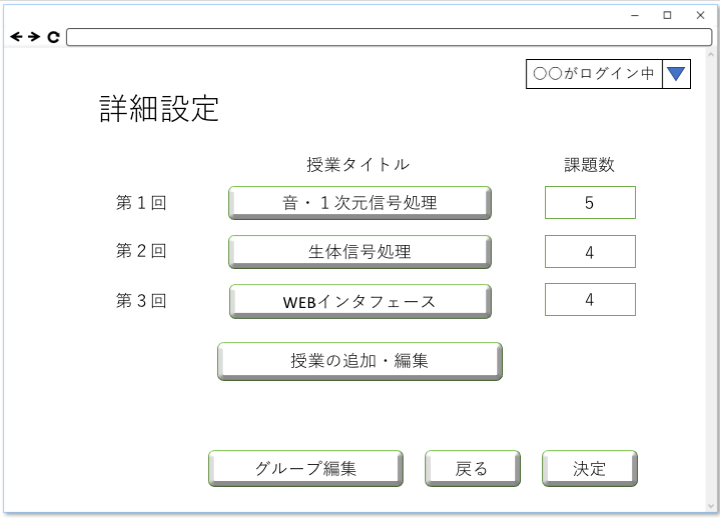
\includegraphics[width=0.7\linewidth,clip]{./img/12.png}
    \caption{詳細設定画面2のイメージ図}\label{fig:12}
  \end{center}
\end{figure}

\newpage

\subsection{詳細設定画面3}
\subsubsection{画面の概要}
% 画面の概要
この画面は、授業回ごとに課題の内容や、「進捗確認画面」で表示される課題名などを設定する画面です。
図\ref{fig:13}にイメージ図を示します。

\subsubsection{操作説明}
% 操作説明
画面左側に「詳細設定画面1」で入力した、課題数分の課題内容を入力するテキストボックスが表示されます。
そのテキストボックス内に課題の内容を入力することで課題内容を設定できます。
画面右側には、進捗確認画面や質問の確認などでカテゴリとして表示される課題名を入力できます。
「決定」ボタンを押すことで内容が確定され、「詳細設定画面2」に戻ります。

\begin{figure}[htbp]
  \begin{center}
    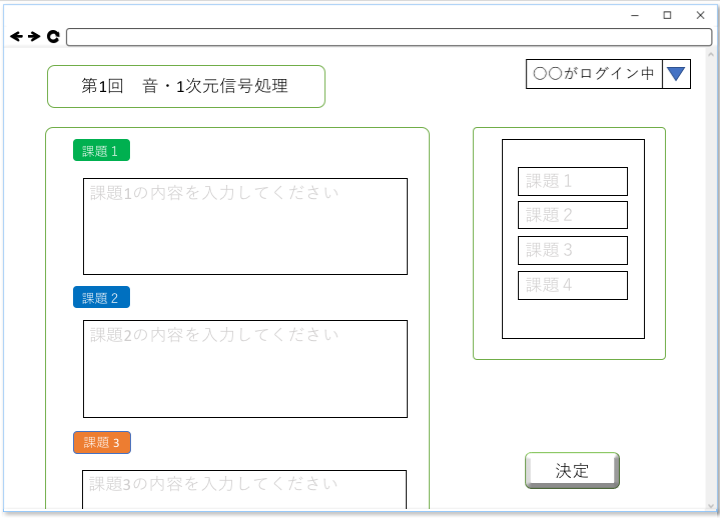
\includegraphics[width=0.7\linewidth,clip]{./img/13.png}
    \caption{詳細設定画面3のイメージ図}\label{fig:13}
  \end{center}
\end{figure}

\newpage

\subsection{編集グループ選択画面}
\subsubsection{画面の概要}
% 画面の概要
この画面は、管理者が編集したいグループを選択する画面です。
また、グループの新規作成を行うこともできます。
図\ref{fig:14}にイメージ図を示します。

\subsubsection{操作説明}
% 操作説明
グループ名のボタンを押すことで、グループの詳細ウィンドウが表示され、「編集」ボタンを押すことで、
そのグループの「グループ編集情報画面」に遷移します。
また、「新規グループ作成」ボタンを押すことで、グループを作成することができます。

\begin{figure}[htbp]
  \begin{center}
    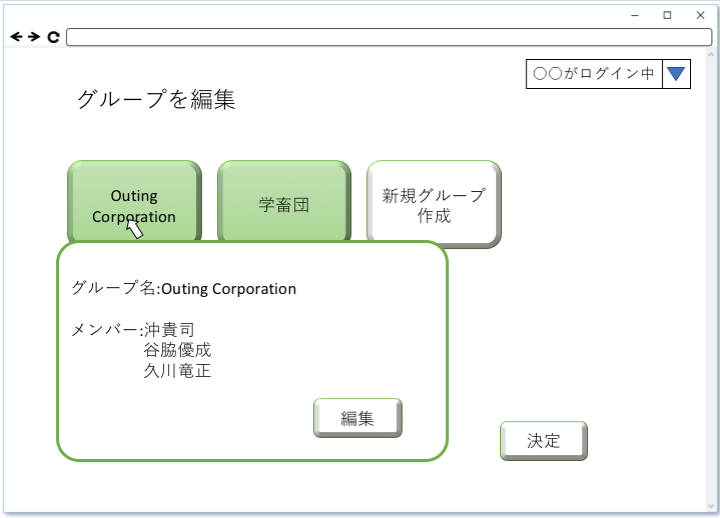
\includegraphics[width=0.7\linewidth,clip]{./img/14.png}
    \caption{編集グループ選択画面のイメージ図}\label{fig:14}
  \end{center}
\end{figure}

\newpage

\subsection{グループ情報編集画面}
\subsubsection{画面の概要}
% 画面の概要
この画面は、管理者が作成されているグループ名の編集および、グループやユーザの削除が行える画面です。
図\ref{fig:15}にイメージ図を示します。

\subsubsection{操作説明}
% 操作説明
グループ名が記載されている部分はテキストを直接編集することができます。
ユーザやグループ自体を削除する場合は、削除対象の右にあるチェックボックスにチェックを入れて、「削除」ボタンを押すことで削除を行うことができます。
最後に「決定」ボタンを押すことで、編集内容を保存し「編集グループ選択画面」に遷移します。

\begin{figure}[htbp]
  \begin{center}
    
\includegraphics[width=0.7\linewidth,clip]{./img/15.png}
    \caption{グループ情報編集画面のイメージ図}\label{fig:15}
  \end{center}
\end{figure}

\newpage

\subsection{管理者用の授業回選択画面}
\subsubsection{画面の概要}
% 画面の概要
この画面は、使用したい授業の回を選択する画面です。
図\ref{fig:16}にイメージ図を示します。

\subsubsection{操作説明}
% 操作説明
授業タイトルのボタンを押すことで、その回の授業の「進捗確認画面」に遷移します。
「質問閲覧・編集」ボタンを押すことで、「質問閲覧・編集画面1」に遷移します。

\begin{figure}[htbp]
  \begin{center}
    
\includegraphics[width=0.7\linewidth,clip]{./img/16.png}
    \caption{管理者用の授業回選択画面のイメージ図}\label{fig:16}
  \end{center}
\end{figure}

\newpage

\subsection{質問閲覧・編集画面1}
\subsubsection{画面の概要}
% 画面の概要
この画面は、質問閲覧・編集を行いたい授業が行われた年度を選択する画面です。
図\ref{fig:17}にイメージ図を示します。

\subsubsection{操作説明}
% 操作説明
年度の書かれたボタンを押すことで、その年度に開かれた授業が回ごとに並んでいる「質問閲覧・編集画面2」に遷移します。

\begin{figure}[htbp]
  \begin{center}
    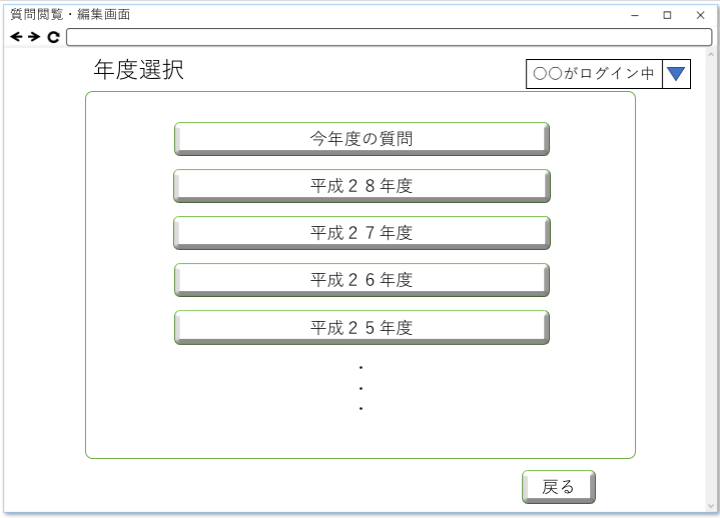
\includegraphics[width=0.7\linewidth,clip]{./img/17.png}
    \caption{質問閲覧・編集画面1のイメージ図}\label{fig:17}
  \end{center}
\end{figure}

\newpage

\subsection{質問閲覧・編集画面2}
\subsubsection{画面の概要}
% 画面の概要
この画面は、質問の閲覧・編集を行いたい授業回を選択する画面です。
図\ref{fig:18}にイメージ図を示します。

\subsubsection{操作説明}
% 操作説明
質問の閲覧や編集を行いたい授業回が書かれているボタンをクリックすることで、
その授業回の「質問閲覧・編集画面3」に遷移します。

\begin{figure}[htbp]
  \begin{center}
    
\includegraphics[width=0.7\linewidth,clip]{./img/18.png}
    \caption{質問閲覧・編集画面2のイメージ図}\label{fig:18}
  \end{center}
\end{figure}

\newpage

\subsection{質問閲覧・編集画面3}
\subsubsection{画面の概要}
% 画面の概要
この画面は、データベースに蓄積されている質問を閲覧・編集できる画面です。
図\ref{fig:19}にイメージ図を示します。

\subsubsection{操作説明}
% 操作説明
質問内容や回答を直接クリックすると編集することができるようになります。
また、非公開のチェックボックスによって学生へその質問を公開するかどうかを選択することができます。
「削除」ボタンでは、その質問自体を削除することができます。

% \begin{figure}[htbp]
  % \begin{center}
    % 
\includegraphics[width=1\linewidth,clip]{./img/19.png}
    % \caption{質問閲覧・編集画面3のイメージ図}\label{fig:19}
  % \end{center}
% \end{figure}

% \begin{figure}[htbp]
  % \begin{center}
    % 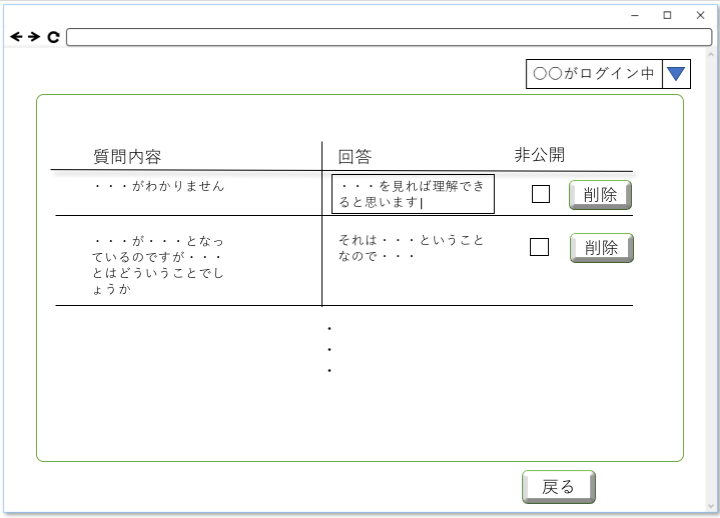
\includegraphics[width=1\linewidth,clip]{./img/000.png}
    % \caption{質問閲覧・編集画面3のイメージ図(質問機能のみ)}\label{fig:000}
  % \end{center}
% \end{figure}

\begin{figure}[htbp]
 \begin{minipage}{0.5\hsize}
  \begin{center}
   
\includegraphics[width=1\linewidth,clip]{./img/19.png}
  \end{center}

 \end{minipage}
 \begin{minipage}{0.5\hsize}
  \begin{center}
   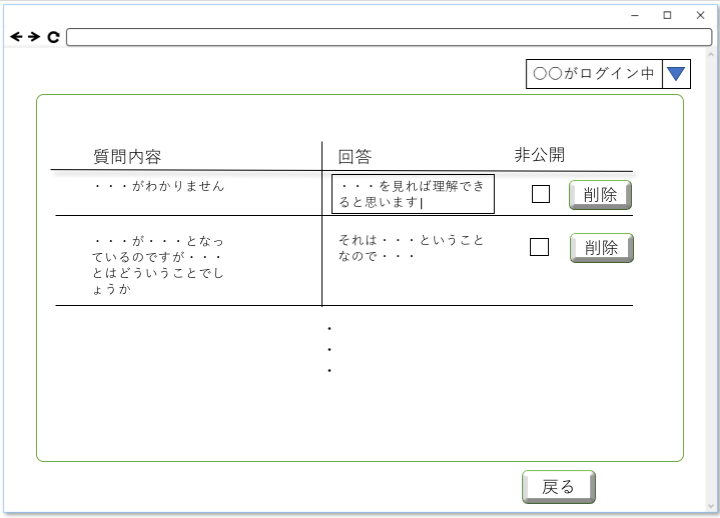
\includegraphics[width=1\linewidth,clip]{./img/000.png}
  \end{center}
  %\caption{質問閲覧・編集画面3のイメージ図(質問機能のみ)}\label{fig:000}
 \end{minipage}
 \caption{質問閲覧・編集画面3のイメージ図}\label{fig:19}
\end{figure}

\newpage

\subsection{進捗確認画面}
\subsubsection{画面の概要}
% 画面の概要
この画面は、授業時に使用される学生の課題の進捗状況を確認する画面です。
図\ref{fig:20}にグループでのイメージ図を示します。
図\ref{fig:22}に個人でのイメージ図を示します。

\subsubsection{操作説明}
% 操作説明
表の形式でユーザごとの進捗が表示されており、氏名の横に課題ごとの進捗が表示されます。%氏名の横かな〜
また、学生から質問があると、その学生の一番右側の状態の欄に黄色のアイコンが表示され、
課題の確認の場合は緑色のアイコン、緊急の場合は赤色のアイコンが表示されます。
画面右下の「課題編集」ボタンを押すことで、今開講している授業の課題内容の編集が行える、「詳細設定画面3」に遷移します。
表内を押すと、その押した行にあるユーザからの質問確認が行えるウィンドウが開き、そのウィンドウの「回答」ボタンを押すことで、%行の
「質問回答画面」に遷移します。

% \begin{figure}[phtbp]
  % \begin{center}
    % 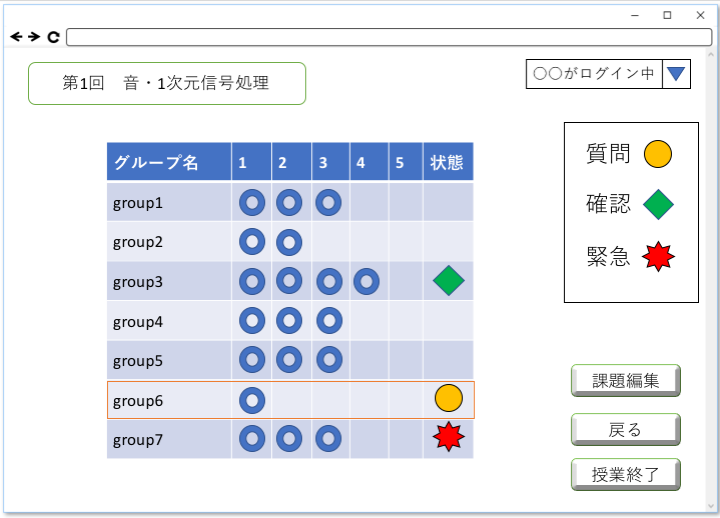
\includegraphics[width=1\linewidth,clip]{./img/20.png}
    % \caption{進捗確認画面(グループ)のイメージ図1}\label{fig:20}
  % \end{center}
% \end{figure}

% \begin{figure}[phtbp]
  % \begin{center}
    % 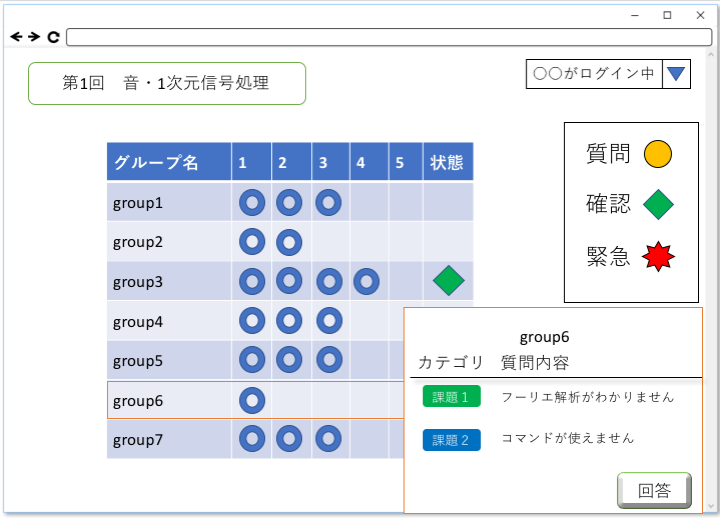
\includegraphics[width=1\linewidth,clip]{./img/21.png}
    % \caption{進捗確認画面(グループ)のイメージ図2}\label{fig:21}
  % \end{center}
% \end{figure}

\begin{figure}[htbp]
 \begin{minipage}{0.5\hsize}
  \begin{center}
   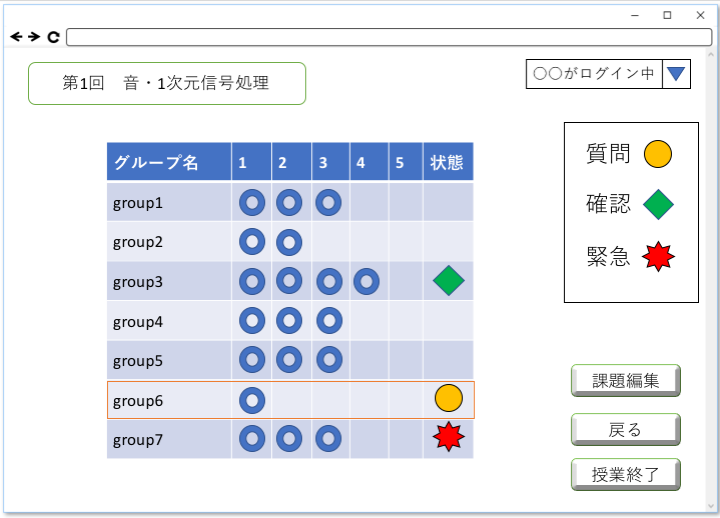
\includegraphics[width=1\linewidth,clip]{./img/20.png}
  \end{center}

 \end{minipage}
 \begin{minipage}{0.5\hsize}
  \begin{center}
   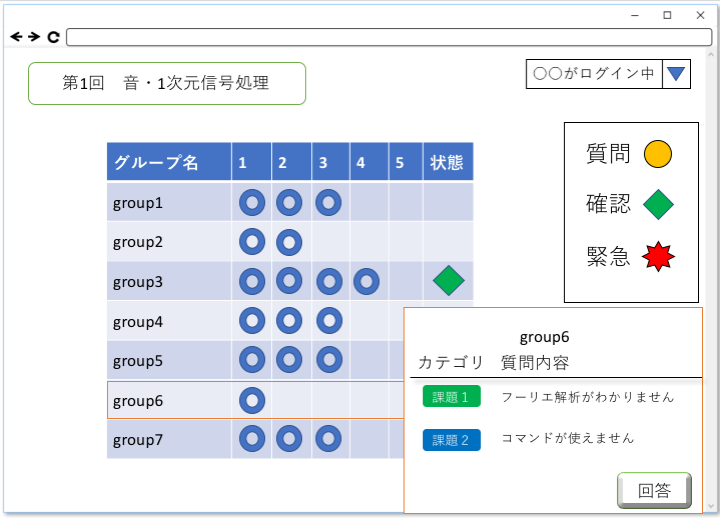
\includegraphics[width=1\linewidth,clip]{./img/21.png}
  \end{center}
  %\caption{進捗確認画面(グループ)のイメージ図2}\label{fig:21}
 \end{minipage}
 \caption{進捗確認画面(グループ)のイメージ図1}\label{fig:20}
\end{figure}

% \begin{figure}[phtbp]
  % \begin{center}
    % 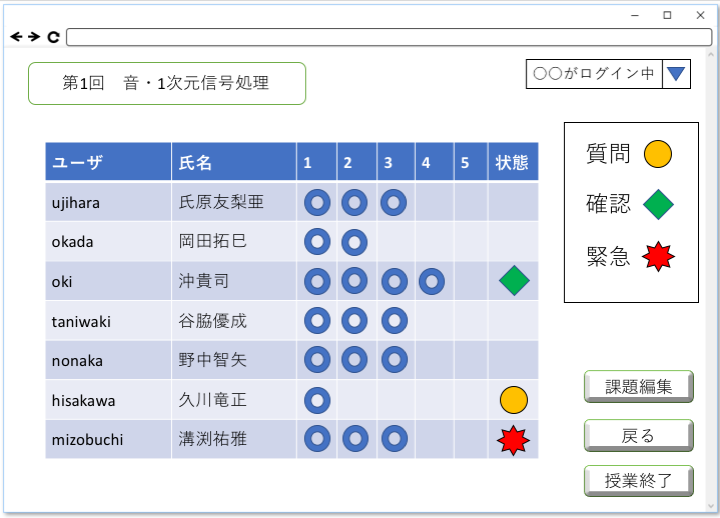
\includegraphics[width=1\linewidth,clip]{./img/22.png}
    % \caption{進捗確認画面(個人)のイメージ図1}\label{fig:22}
  % \end{center}
% \end{figure}

% \begin{figure}[phtbp]
  % \begin{center}
    % 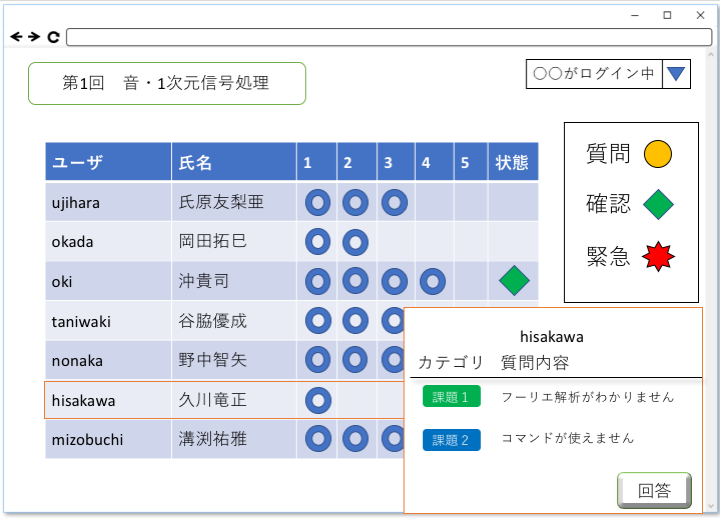
\includegraphics[width=1\linewidth,clip]{./img/23.png}
    % \caption{進捗確認画面(個人)のイメージ図2}\label{fig:23}
  % \end{center}
% \end{figure}

\begin{figure}[htbp]
 \begin{minipage}{0.5\hsize}
  \begin{center}
   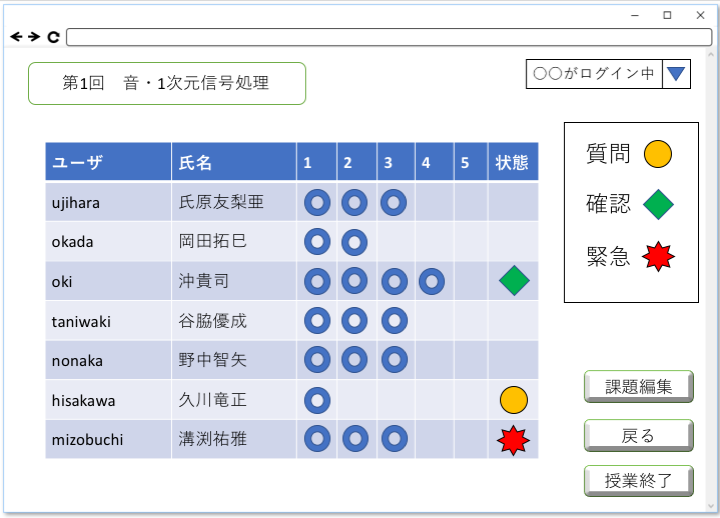
\includegraphics[width=1\linewidth,clip]{./img/22.png}
  \end{center}

 \end{minipage}
 \begin{minipage}{0.5\hsize}
  \begin{center}
   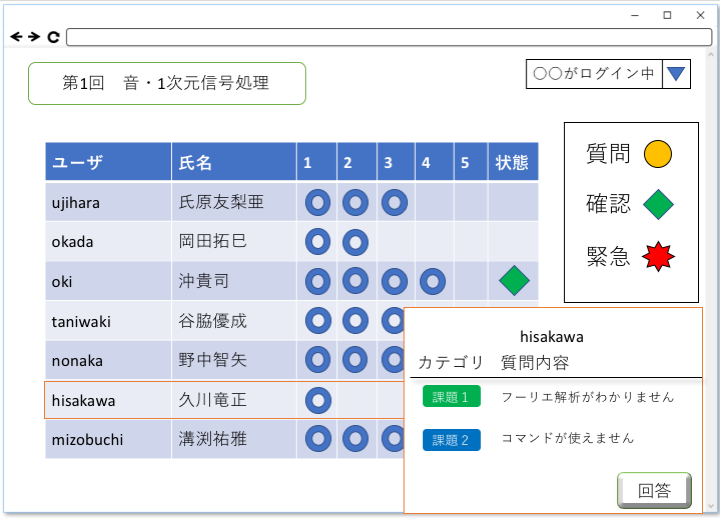
\includegraphics[width=1\linewidth,clip]{./img/23.png}
  \end{center}
  %\caption{進捗確認画面(個人)のイメージ図2}\label{fig:23}
 \end{minipage}
 \caption{進捗確認画面(個人)のイメージ図1}\label{fig:22}
\end{figure}

\newpage

\subsection{質問回答画面}
\subsubsection{画面の概要}
% 画面の概要
この画面には、左側にグループ名と、そのグループからの質問が表示されています。
図\ref{fig:24}にイメージ図を示します。

\subsubsection{操作説明}
% 操作説明
質問へ回答をしたい場合、その質問が表示されている部分を選択した後、右側にある回答記入欄に回答を記入し、「回答」ボタンをクリックすることで送信します。
質問や回答の内容は他の学生も閲覧することが可能となっており、その質問や回答の内容を公開するかどうかは、質問の横にある非公開のチェックボックスによって設定ができます。

% \begin{figure}[phtbp]
  % \begin{center}
    % 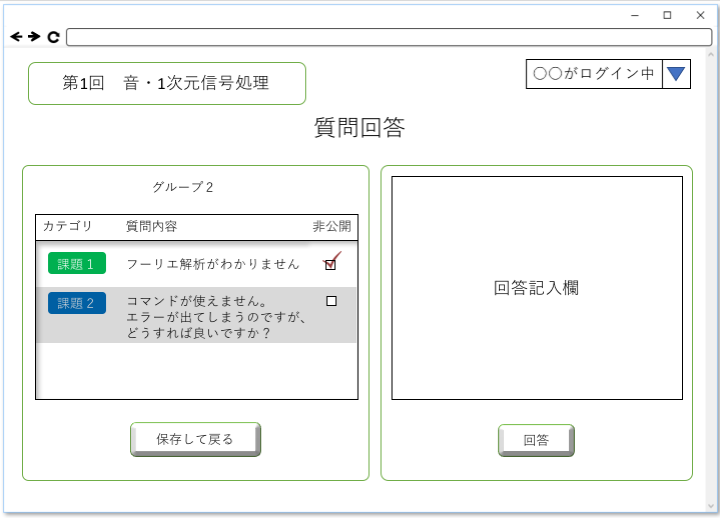
\includegraphics[width=1\linewidth,clip]{./img/24.png}
    % \caption{質問回答画面(課題に対する質問)}\label{fig:24}
  % \end{center}
% \end{figure}

% \begin{figure}[phtbp]
  % \begin{center}
    % 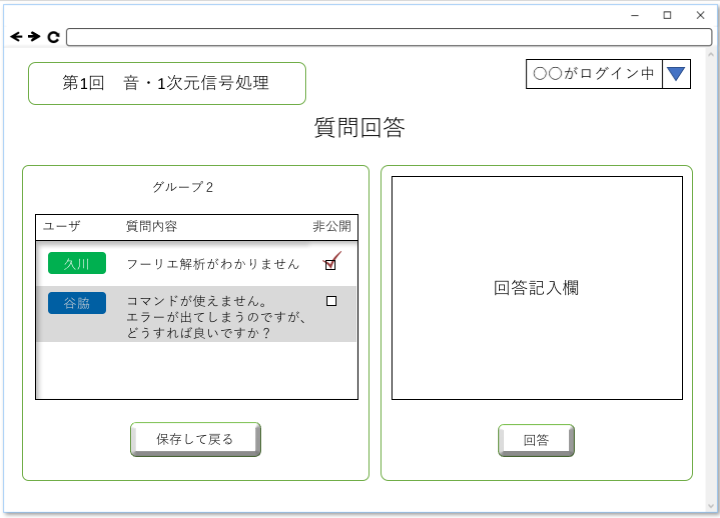
\includegraphics[width=1\linewidth,clip]{./img/25.png}
    % \caption{質問回答画面(授業に対する質問)}\label{fig:25}
  % \end{center}
% \end{figure}

\begin{figure}[htbp]
 \begin{minipage}{0.5\hsize}
  \begin{center}
   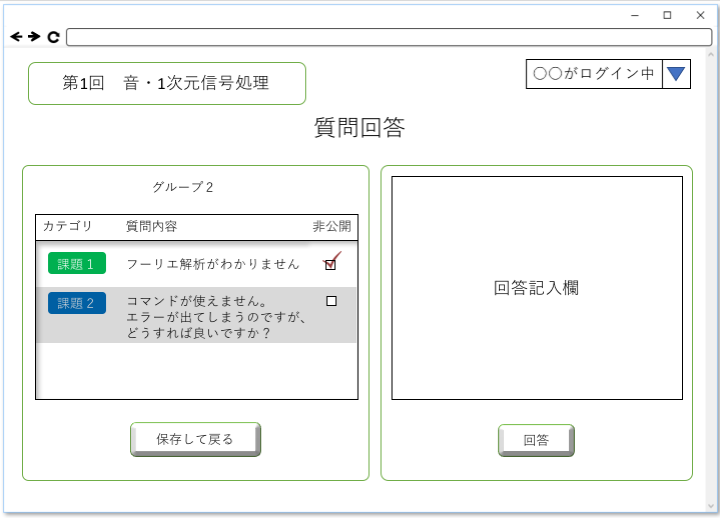
\includegraphics[width=1\linewidth,clip]{./img/24.png}
  \end{center}

 \end{minipage}
 \begin{minipage}{0.5\hsize}
  \begin{center}
   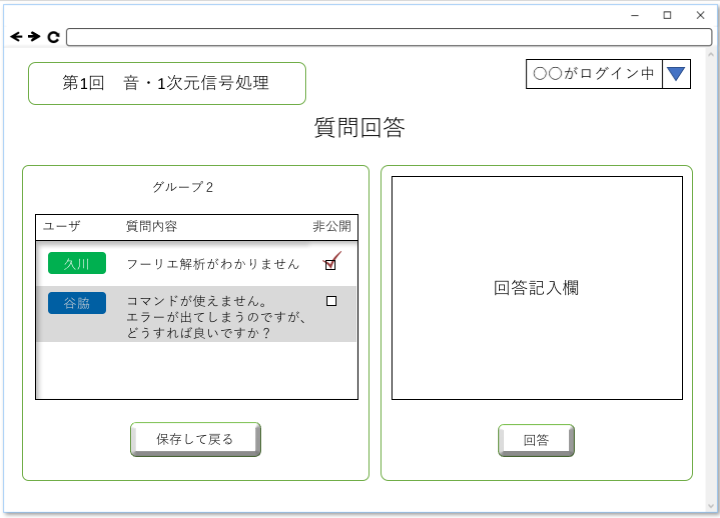
\includegraphics[width=1\linewidth,clip]{./img/25.png}
  \end{center}
  %\caption{質問回答画面(課題に対する質問)のイメージ図}\label{fig:25}
 \end{minipage}
 \caption{質問回答画面(課題に対する質問)のイメージ図}\label{fig:24}
\end{figure}

\newpage

\subsection{グループ参加・作成画面}
\subsubsection{画面の概要}
% 画面の概要
この画面は、開講されている授業がグループで行う授業であり、まだどのグループにも参加していない場合に、ログインすると表示される画面です。
この画面では、すでに作成されているグループへの参加と、新規グループの作成が行えます。
図\ref{fig:26}にイメージ図を示します。

\subsubsection{操作説明}
% 操作説明

作成されているグループに参加する場合、参加したいグループ名の書かれたボタンを押します。
するとウィンドウが表示され、中にグループ名と現状参加しているメンバーが表示されるので、
内容を確認して参加する場合、「参加」ボタンを押してグループへの参加を完了します。
グループを間違えた場合は、ウィンドウ外をクリックして画面を閉じます。

グループを作成する場合、「新規グループ作成」ボタンを押します。
ウィンドウが表示されるので、グループ名を記入し、「作成」ボタンを押して作成を完了します。

% \begin{figure}[phtbp]
  % \begin{center}
    % 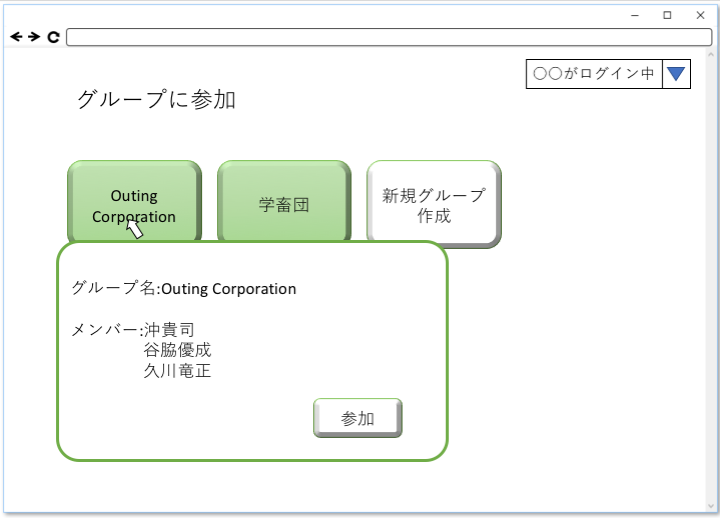
\includegraphics[width=1\linewidth,clip]{./img/26.png}
    % \caption{グループ参加・作成画面のグループ参加イメージ図}\label{fig:26}
  % \end{center}
% \end{figure}

% \begin{figure}[phtbp]
  % \begin{center}
    % 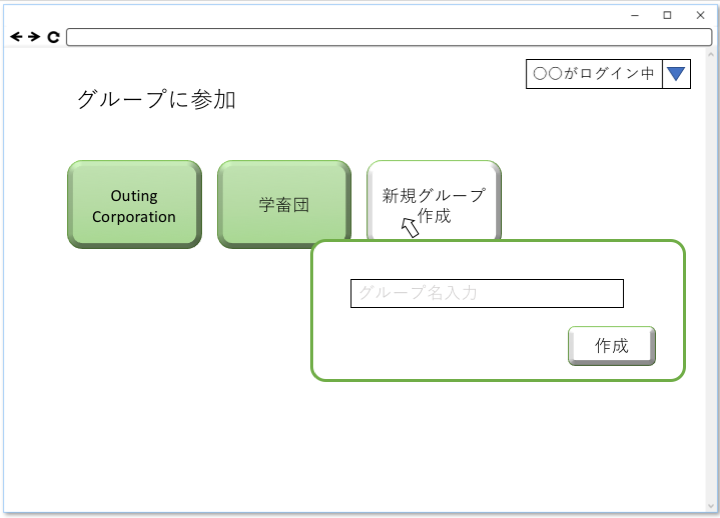
\includegraphics[width=1\linewidth,clip]{./img/27.png}
    % \caption{グループ参加・作成画面のグループ作成イメージ図}\label{fig:27}
  % \end{center}
% \end{figure}

\begin{figure}[htbp]
 \begin{minipage}{0.5\hsize}
  \begin{center}
   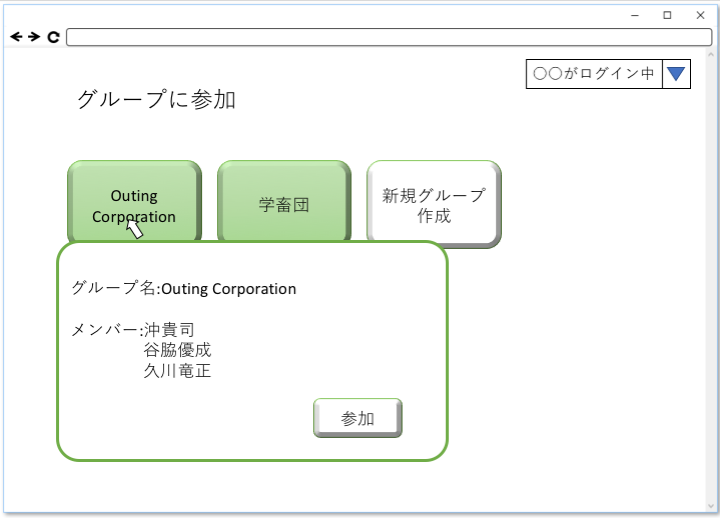
\includegraphics[width=1\linewidth,clip]{./img/26.png}
  \end{center}

 \end{minipage}
 \begin{minipage}{0.5\hsize}
  \begin{center}
   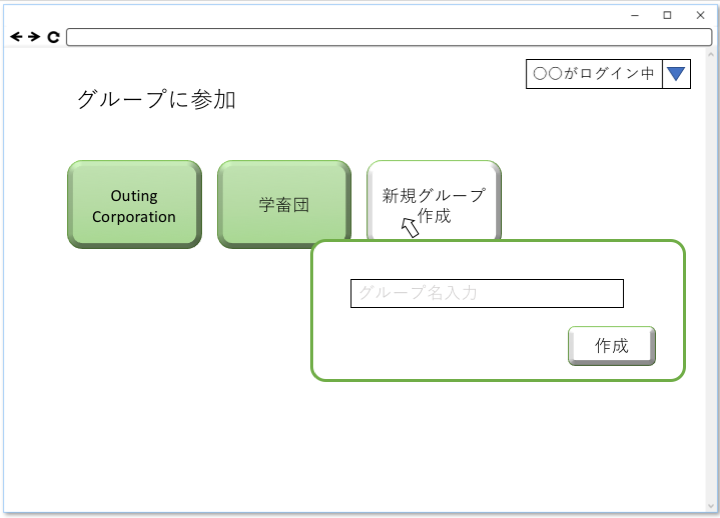
\includegraphics[width=1\linewidth,clip]{./img/27.png}
  \end{center}
  %\caption{グループ参加・作成画面のグループ作成イメージ図}\label{fig:27}
 \end{minipage}
 \caption{グループ参加・作成画面のグループ参加イメージ図}\label{fig:26}
\end{figure}

\newpage

\subsection{学生用のホーム画面}
\subsubsection{画面の概要}
% 画面の概要
この画面は、学生側のホーム画面です。
この画面では、今年度の質問を確認したり、進捗状況を管理者側に送信したりできます。
画面上部に授業名が表示されており、その下に質問確認欄と進捗状況入力欄があります。
左側の質問確認欄には、受講中の内容に関する質問が表示されており、カテゴリ順に並べられています。
ログイン時に授業が開講されていない場合はエラーが表示されます。
図\ref{fig:28}、\ref{fig:00}にイメージ図を示します。

\subsubsection{操作説明}
% 操作説明
過去の質問を確認する場合、質問確認欄にある「過去の質問」ボタンを押して「学生用の年度選択画面」に遷移します。
質問をする場合、質問確認欄にある「質問をする」ボタンを押して「質問入力画面」に遷移します。
進捗状況を管理者側に送信する場合、進捗状況入力欄にあるチェックボックスに終わった課題分チェックをつけて「更新」ボタンを押して更新を行います。
全ての課題を終えて管理者側に確認を行ってもらいたい場合、「確認」ボタンを押します。

% \begin{figure}[phtbp]
  % \begin{center}
    % 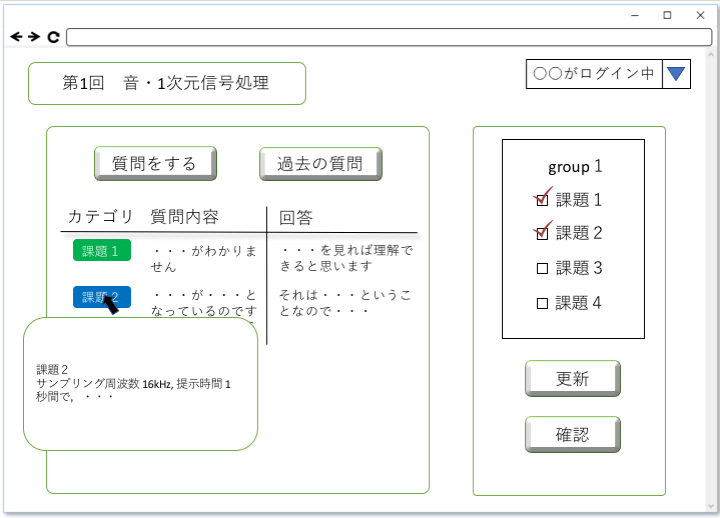
\includegraphics[width=1\linewidth,clip]{./img/28.png}
    % \caption{学生用のホーム画面のイメージ図}\label{fig:28}
  % \end{center}
% \end{figure}

% \begin{figure}[phtbp]
  % \begin{center}
    % 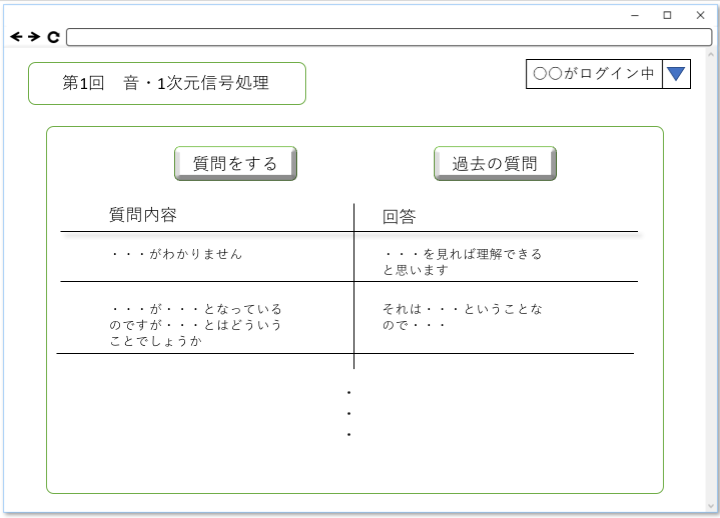
\includegraphics[width=1\linewidth,clip]{./img/29.png}
    % \caption{学生用のホーム画面のイメージ図(質問機能のみ)}\label{fig:29}
  % \end{center}
% \end{figure}

\begin{figure}[htbp]
 \begin{minipage}{0.5\hsize}
  \begin{center}
   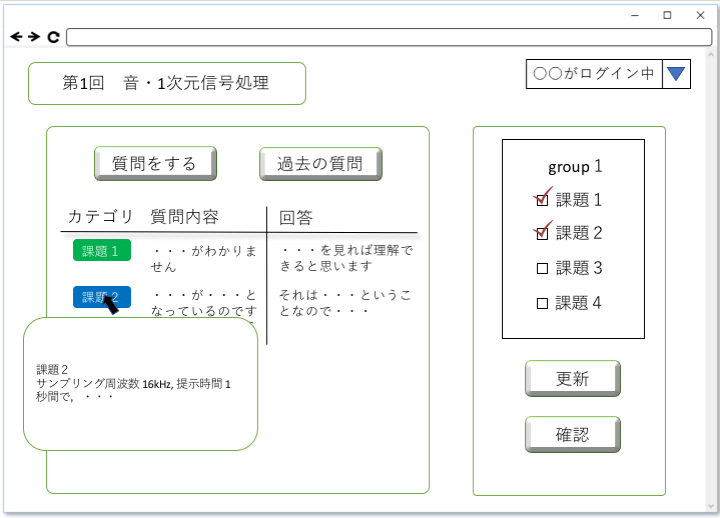
\includegraphics[width=1\linewidth,clip]{./img/28.png}
  \end{center}

 \end{minipage}
 \begin{minipage}{0.5\hsize}
  \begin{center}
   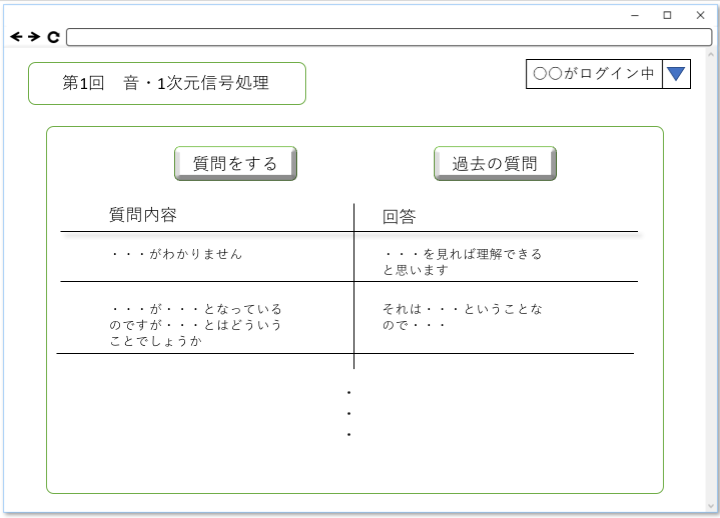
\includegraphics[width=1\linewidth,clip]{./img/29.png}
  \end{center}
  %\caption{学生用のホーム画面のイメージ図(質問機能のみ)}\label{fig:29}
 \end{minipage}
 \caption{学生用のホーム画面のイメージ図}\label{fig:28}
\end{figure}

\begin{figure}[htbp]
  \begin{center}
    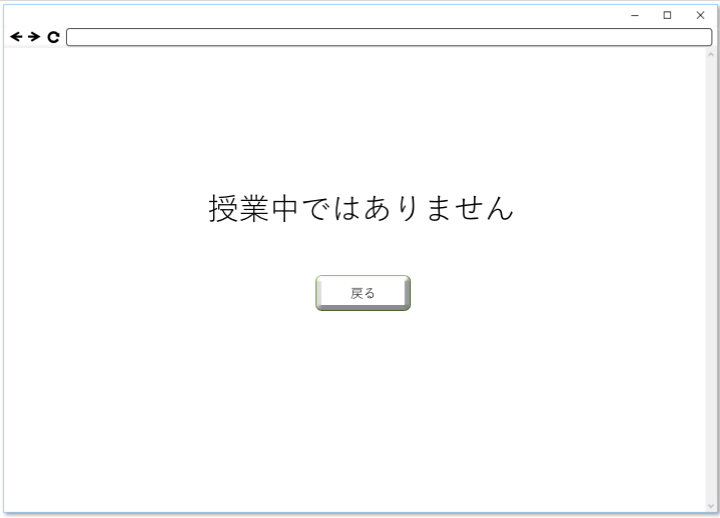
\includegraphics[width=0.5\linewidth,clip]{./img/00.png}
    \caption{学生用のホーム画面のエラー表示イメージ図}\label{fig:00}
  \end{center}
\end{figure}

\newpage

\subsection{学生用の年度選択画面}
\subsubsection{画面の概要}
% 画面の概要
この画面は、学生側が過去の質問を確認する際に、どの年度に出た質問を確認するのか選択する画面です。
図\ref{fig:30}にイメージ図を示します。

\subsubsection{操作説明}
% 操作説明
年度のボタンを押すと、その年度の「学生用の授業回選択画面」に遷移します。
「今年度の質問」ボタンを押すと今年度の質問が表示されている「学生用のホーム画面」に戻ります。

% \begin{figure}[phtbp]
  % \begin{center}
    % 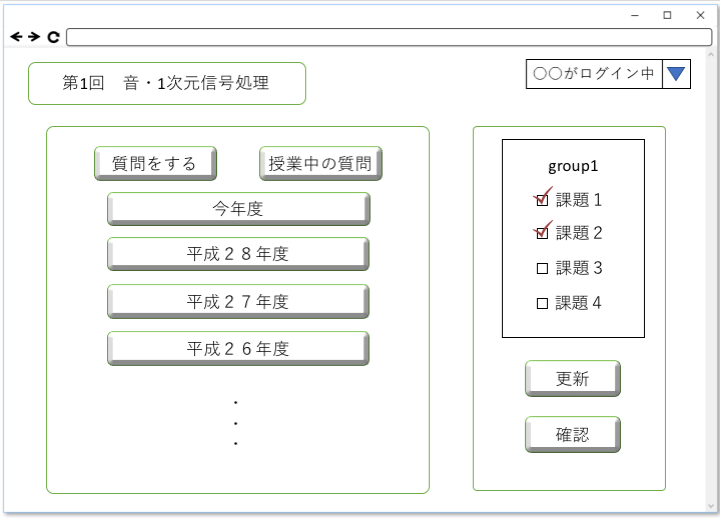
\includegraphics[width=1\linewidth,clip]{./img/30.png}
    % \caption{学生用の年度選択画面のイメージ図}\label{fig:30}
  % \end{center}
% \end{figure}

% \begin{figure}[phtbp]
  % \begin{center}
    % \includegraphics[width=1\linewidth,clip]{./img/31.png}
    % \caption{学生用の年度選択画面のイメージ図(質問機能のみの場合)}\label{fig:31}
  % \end{center}
% \end{figure}

\begin{figure}[htbp]
 \begin{minipage}{0.5\hsize}
  \begin{center}
   \includegraphics[width=1\linewidth,clip]{./img/30.png}
  \end{center}

 \end{minipage}
 \begin{minipage}{0.5\hsize}
  \begin{center}
   \includegraphics[width=1\linewidth,clip]{./img/31.png}
  \end{center}
  %\caption{学生用の年度選択画面のイメージ図(質問機能のみの場合)}\label{fig:31}
 \end{minipage}
 \caption{学生用の年度選択画面のイメージ図}\label{fig:30}
\end{figure}

\newpage

\subsection{学生用の授業回選択画面}
\subsubsection{画面の概要}
% 画面の概要
この画面は、学生側が選択した質問を確認したい年度に対して、どの授業回か選択する画面です。
図\ref{fig:32}にイメージ図を示します。

\subsubsection{操作説明}
% 操作説明
授業回を選択するとその回の授業で出た質問が表示される「学生用の過去質問画面」に遷移します。
「年度選択」ボタンを押すと「学生用の年度選択画面」に戻ります。

% \begin{figure}[phtbp]
  % \begin{center}
    % \includegraphics[width=1\linewidth,clip]{./img/32.png}
    % \caption{学生用の授業回選択画面のイメージ図}\label{fig:32}
  % \end{center}
% \end{figure}

% \begin{figure}[phtbp]
  % \begin{center}
    % \includegraphics[width=1\linewidth,clip]{./img/33.png}
    % \caption{学生用の授業回選択画面のイメージ図(質問機能のみ)}\label{fig:33}
  % \end{center}
% \end{figure}

\begin{figure}[htbp]
 \begin{minipage}{0.5\hsize}
  \begin{center}
   \includegraphics[width=1\linewidth,clip]{./img/32.png}
  \end{center}

 \end{minipage}
 \begin{minipage}{0.5\hsize}
  \begin{center}
   \includegraphics[width=1\linewidth,clip]{./img/33.png}
  \end{center}
  %\caption{学生用の授業回選択画面のイメージ図(質問機能のみの場合)}\label{fig:33}
 \end{minipage}
 \caption{学生用の授業回選択画面のイメージ図}\label{fig:32}
\end{figure}

\newpage

\subsection{学生用の過去質問画面}
\subsubsection{画面の概要}
% 画面の概要
この画面は、学生側が選択した条件に合わせて過去の質問が表示される画面です。
基本的に「学生用のホーム画面」と表示されていることは変わりませんが、「授業回選択」ボタンを押すことで
「学生用の授業回選択画面」に遷移します。
図\ref{fig:34}にイメージ図を示します。

\subsubsection{操作説明}
% 操作説明
「質問をする」ボタンを押すと他の画面同様、「質問入力画面」に移動します。
「授業回選択」ボタンを押すと、「学生用の授業回選択画面」へ戻ります。
2つのボタンの下には、選択した授業回について過去に出た質問が表示されます。

% \begin{figure}[phtbp]
  % \begin{center}
    % \includegraphics[width=1\linewidth,clip]{./img/34.png}
    % \caption{学生用の過去質問画面のイメージ図}\label{fig:34}
  % \end{center}
% \end{figure}

% \begin{figure}[phtbp]
  % \begin{center}
    % \includegraphics[width=1\linewidth,clip]{./img/35.png}
    % \caption{学生用の過去質問画面のイメージ図(質問機能のみ)}\label{fig:35}
  % \end{center}
% \end{figure}

\begin{figure}[htbp]
 \begin{minipage}{0.5\hsize}
  \begin{center}
   \includegraphics[width=1\linewidth,clip]{./img/34.png}
  \end{center}

 \end{minipage}
 \begin{minipage}{0.5\hsize}
  \begin{center}
   \includegraphics[width=1\linewidth,clip]{./img/35.png}
  \end{center}
  %\caption{学生用の過去質問画面のイメージ図(質問機能のみの場合)}\label{fig:35}
 \end{minipage}
 \caption{学生用の過去質問画面のイメージ図}\label{fig:34}
\end{figure}

\newpage



\subsection{質問入力画面}
\subsubsection{画面の概要}
% 画面の概要
この画面は、学生側が管理者側に送信する質問内容を入力する画面です。
図\ref{fig:36}にイメージ図を示します。

\subsubsection{操作説明}
% 操作説明
まず画面上部の三角を押して、どの課題に対して質問をするのか選びます。
次にその下の質問入力欄に質問内容を入力して、「質問」ボタンを押します。
PCに問題が起きた時などの緊急案件の場合は課題選択のところに用意してあるその他を選んでいただき、
内容を書いて「緊急」ボタンを押していただきます。
2つのどのボタンを押しても管理者に内容を送信後、1つ手前の画面に戻ります。
課題がない授業の場合は、質問記入欄のみが画面に表示されます。
% \begin{figure}[phtbp]
  % \begin{center}
    % \includegraphics[width=1\linewidth,clip]{./img/36.png}
    % \caption{質問入力画面のイメージ図}\label{fig:36}
  % \end{center}
% \end{figure}

% \begin{figure}[phtbp]
  % \begin{center}
    % \includegraphics[width=1\linewidth,clip]{./img/37.png}
    % \caption{質問入力画面のイメージ図(質問機能のみ)}\label{fig:37}
  % \end{center}
% \end{figure}

\begin{figure}[htbp]
 \begin{minipage}{0.5\hsize}
  \begin{center}
   \includegraphics[width=1\linewidth,clip]{./img/36.png}
  \end{center}

 \end{minipage}
 \begin{minipage}{0.5\hsize}
  \begin{center}
   \includegraphics[width=1\linewidth,clip]{./img/37.png}
  \end{center}
  %\caption{質問入力画面のイメージ図(質問機能のみの場合)}\label{fig:37}
 \end{minipage}
 \caption{質問入力画面のイメージ図}\label{fig:36}
\end{figure}

\newpage

\newpage
\section{データベースの設計}
本システムで使用するデータベースMySQLのテーブルについて示します。また、ERモデルで表したER図式を図\ref{fig:ER}で示します。
\begin{figure}[h]
	\begin{center}
	\includegraphics[width=1\linewidth,clip]{./img/er.png}
	\caption{実体関連図式}
	\label{fig:ER}
	\end{center}
\end{figure}

\newpage
\subsection{ユーザテーブル}
本システム利用者のユーザ情報を格納します。権限が「学生」であるユーザ情報は、登録日から設定した年が経過すると削除されます。各フィールドの概要は以下の通りです。また、ユーザテーブルの詳細は表\ref{ユーザテーブル}で示します。
\begin{itemize}
	\item ユーザ番号(USER\_NO):\\ユーザテーブルの主キー
	\item ユーザID(USER\_ID):\\システムにおいてユーザを一意に定める名前
	\item パスワード(PASSWORD):\\ユーザの識別・確認に用いるパスワード
	\item 氏名(USER\_NAME):\\ユーザ本人の名前
	\item 権限(AUTHORITY):\\ユーザに「教員」、「アシスタント」または「学生」のいずれかの権限を与える
\end{itemize}

	\begin{table}[h]
		\centering
		\caption{ユーザテーブル(TB\_USER)}
		\label{ユーザテーブル}
		\begin{tabular}{|l|l|l|c|l|}
		\hline
		フィールド & 型  & 外部キー & Null & オプション\\ \hline\hline
		\ul{ユーザ番号} & \begin{tabular}[c]{@{}l@{}}INT\\ UNSIGNED\end{tabular} &  & No & AUTO\_INCREMENT\\ \hline
		ユーザID & VARCHAR(32) & & No & UNIQUE\\ \hline
		パスワード & VARCHAR(64) & & No & \\ \hline
		氏名 & VARCHAR(16) &  & No  &\\ \hline
		権限 & ENUM & & No & \\ \hline
		\end{tabular}
	\end{table}

\newpage

\subsection{履修者テーブル}
受講するユーザ情報を格納します。各フィールドの概要は以下の通りです。また、履修者テーブルの詳細は表\ref{履修者テーブル}で示します。
\begin{itemize}
	\item 開講年度番号(LECTURE\_YEAR\_NO):\\何年度の何の授業であるかを示す
	\item ユーザ番号(USER\_NO):\\授業を履修する学生ユーザ
\end{itemize}

	\begin{table}[h]
		\centering
		\caption{履修者テーブル(TB\_STUDENT)}
		\label{履修者テーブル}
		\begin{tabular}{|l|l|l|c|l|}
		\hline
		フィールド & 型 & 外部キー & Null & オプション \\ \hline\hline
		開講年度番号 & \begin{tabular}[c]{@{}l@{}}INT\\ UNSIGNED\end{tabular} & 開講年度 & No & \\ \hline
		ユーザ番号 & \begin{tabular}[c]{@{}l@{}}INT\\ UNSIGNED\end{tabular} & ユーザ & No & \\ \hline
		\end{tabular}
	\end{table}

\subsection{グループテーブル}
授業のために作成されたグループ情報を格納します。各フィールドの概要は以下の通りです。また、グループテーブルの詳細は表\ref{グループテーブル}で示します。
\begin{itemize}
	\item グループ番号(GROUP\_NO):\\グループテーブルの主キー
	\item グループ名(GROUP\_NAME):\\グループの名前
	\item 開講年度番号(LECTURE\_YEAR\_NO):\\何年度の何の授業のために作成されたかを示す
\end{itemize}

	\begin{table}[h]
		\centering
		\caption{グループテーブル(TB\_GROUP)}
		\label{グループテーブル}
		\begin{tabular}{|l|l|l|c|l|}
		\hline
		フィールド & 型 & 外部キー & Null & オプション\\ \hline\hline
		\ul{グループ番号} & \begin{tabular}[c]{@{}l@{}}INT\\ UNSIGNED\end{tabular} & & No & AUTO\_INCREMENT \\ \hline
		グループ名 & VARCHAR(16) & & No & \\ \hline
		開講年度番号 & \begin{tabular}[c]{@{}l@{}}INT\\ UNSIGNED\end{tabular} & 授業 & No & \\ \hline
		\end{tabular}
	\end{table}

\subsection{グループメンバテーブル}
授業のために作成されたグループに所属しているユーザ情報を格納します。各フィールドの概要は以下の通りです。また、グループメンバテーブルの詳細は表\ref{グループメンバテーブル}で示します。
\begin{itemize}
	\item グループ番号(GROUP\_NO):\\何年度の何の授業のために作成されたグループであるかを示す
	\item ユーザ番号(USER\_NO):\\グループに所属している学生
\end{itemize}

	\begin{table}[h]
		\centering
		\caption{グループメンバテーブル(TB\_GROUP\_MEMBER)}
		\label{グループメンバテーブル}
		\begin{tabular}{|l|l|l|c|l|}
		\hline
		フィールド & 型 & 外部キー & Null & オプション\\ \hline\hline
		グループ番号 & \begin{tabular}[c]{@{}l@{}}INT\\ UNSIGNED\end{tabular} & グループ & No & \\ \hline
		ユーザ番号 & \begin{tabular}[c]{@{}l@{}}INT\\ UNSIGNED\end{tabular} & ユーザ & No & \\ \hline
		\end{tabular}
	\end{table}
\subsection{授業テーブル}
本システムを利用する授業の情報を格納します。各フィールドの概要は以下の通りです。また、授業テーブルの詳細は表\ref{授業テーブル}で示します。
\begin{itemize}
	\item 授業番号(LECTURE\_NO):\\授業テーブルの主キー
	\item 授業名(LECTURE\_NAME):\\授業の名前
\end{itemize}

	\begin{table}[h]
		\centering
		\caption{授業テーブル(TB\_LECTURE)}
		\label{授業テーブル}
		\begin{tabular}{|l|l|l|c|l|}
		\hline
		フィールド & 型 & 外部キー & Null & オプション \\ \hline\hline
		\ul{授業番号} & \begin{tabular}[c]{@{}l@{}}INT\\ UNSIGNED\end{tabular} & & No & AUTO\_INCREMENT \\ \hline
		授業名 & VARCHAR(32) & & No & UNIQUE \\ \hline
		\end{tabular}
	\end{table}
\subsection{開講年度テーブル}
開講された年度を含めた授業情報を格納します。各フィールドの概要は以下の通りです。また、開講年度テーブルの詳細は表\ref{開講年度テーブル}で示します。
\begin{itemize}
	\item 開講年度番号(LECTURE\_YEAR\_NO):\\開講年度テーブルの主キー
	\item 授業番号(LECTURE\_NO):\\授業を示す
	\item 開講年度(LECTURE\_YEAR):\\開講された年度を示す
	\item 授業形態(LECTURE\_STYLE):\\授業の進捗を「個人」または「グループ」のどちらで表示するかを示す
\end{itemize}

	\begin{table}[h]
		\centering
		\caption{開講年度テーブル(TB\_LECTURE\_YEAR)}
		\label{開講年度テーブル}
		\begin{tabular}{|l|l|l|c|l|}
		\hline
		フィールド & 型 & 外部キー & Null & オプション \\ \hline\hline
		\ul{開講年度番号} & \begin{tabular}[c]{@{}l@{}}INT\\ UNSIGNED\end{tabular} & & No & AUTO\_INCREMENT \\ \hline
		授業番号 & \begin{tabular}[c]{@{}l@{}}INT\\ UNSIGNED\end{tabular} & 授業 & No & \\ \hline
		開講年度 & \begin{tabular}[c]{@{}l@{}}SMALLINT\\ UNSIGNED\end{tabular} & & No & \\ \hline
		授業形態 & ENUM & & No & \\ \hline
		\end{tabular}
	\end{table}

\subsection{開講回テーブル}
回ごとの授業情報を格納します。各フィールドの概要は以下の通りです。また、開講回テーブルの詳細は表\ref{開講回テーブル}で示します。
\begin{itemize}
	\item 開講回番号(LECTURE\_TIMES\_NO):\\開講回テーブルの主キー
	\item 開講年度番号(LECTURE\_YEAR\_NO):\\何年度の何の授業であるかを示す
	\item 開講回(LECTURE\_TIMES):\\何年度の何の授業の何回目に開講されたかを示す
	\item 授業題目(LECTURE\_TITLE):\\開講された回ごとの授業概要を示す
\end{itemize}

	\begin{table}[h]
		\centering
		\caption{開講回テーブル(TB\_LECTURE\_TIMES)}
		\label{開講回テーブル}
		\begin{tabular}{|l|l|l|c|l|}
		\hline
		フィールド & 型 & 外部キー & Null & オプション \\ \hline\hline
		\ul{開講回番号} & \begin{tabular}[c]{@{}l@{}}INT\\ UNSIGNED\end{tabular} &  & No & AUTO\_INCREMENT \\ \hline
		開講年度番号 & \begin{tabular}[c]{@{}l@{}}INT\\ UNSIGNED\end{tabular} & 開講年度 & No & \\ \hline
		開講回 & \begin{tabular}[c]{@{}l@{}}TINYINT\\ UNSIGNED\end{tabular} & & No & \\ \hline
		授業題目 & VARCHAR(256) & & & \\ \hline
		\end{tabular}
	\end{table}
\subsection{公開テーブル}
現在開講されている授業情報を格納します。各フィールドの概要は以下の通りです。また、公開テーブルの詳細は表\ref{公開テーブル}で示します。
\begin{itemize}
	\item ユーザ番号(USER\_NO):\\講義を開講した管理者を示す
	\item 授業番号(LECTURE\_NO):\\開講されている授業を示す
	\item 開講回番号(LECTURE\_TIMES\_NO):\\開講されている回を示す
\end{itemize}

	\begin{table}[h]
		\centering
		\caption{公開テーブル(TB\_OPEN\_LECTURE)}
		\label{公開テーブル}
		\begin{tabular}{|l|l|l|c|l|}
		\hline
		フィールド & 型 & 外部キー & Null & オプション \\ \hline\hline
		ユーザ番号 & \begin{tabular}[c]{@{}l@{}}INT\\ UNSIGNED\end{tabular} & ユーザ  & & \\ \hline
		授業番号 & \begin{tabular}[c]{@{}l@{}}INT\\ UNSIGNED\end{tabular} & 授業 &  & \\ \hline
		開講回番号 & \begin{tabular}[c]{@{}l@{}}INT\\ UNSIGNED\end{tabular} & 開講回 & No & \\ \hline
		\end{tabular}
	\end{table}

\subsection{課題テーブル}
授業の回ごとに提示する課題情報を格納します。各フィールドの概要は以下の通りです。また、課題テーブルの詳細は表\ref{課題テーブル}で示します。
\begin{itemize}
	\item 課題番号(PROBLEM\_NO):\\課題テーブルの主キー
	\item 開講回番号(LECTURE\_TIMES\_NO):\\何年度の何の授業の何回目の授業であるかを示す
	\item 課題名(PROBLEM\_NAME):\\授業回ごとに提示される課題の番号
	\item 課題内容(PROBLEM\_CONTENT):\\授業回ごとに提示される課題の内容
\end{itemize}

	\begin{table}[h]
		\centering
		\caption{課題テーブル(TB\_PROBLEM)}
		\label{課題テーブル}
		\begin{tabular}{|l|l|l|c|l|}
		\hline
		フィールド & 型 & 外部キー & Null & オプション \\ \hline\hline
		\ul{課題番号} & \begin{tabular}[c]{@{}l@{}}INT\\ UNSIGNED\end{tabular} & & No & AUTO\_INCREMENT \\ \hline
		開講回番号 & \begin{tabular}[c]{@{}l@{}}INT\\ UNSIGNED\end{tabular} & 開講回 & No & \\ \hline
		課題名 & VARCHAR(8) & & No  & \\ \hline
		課題内容 & VARCHAR(512) & & No & \\ \hline
		\end{tabular}
	\end{table}
\subsection{進捗テーブル}
授業回ごとの学生の課題の進捗情報を格納します。進捗情報は授業時間内のみで使用するため、授業終了から一定期間後に格納された情報は削除されます。各フィールドの概要は以下の通りです。また、進捗テーブルの詳細は表\ref{進捗テーブル}で示します。
\begin{itemize}
	\item 進捗番号(PROGRESS_NO):\\進捗テーブルの主キー
	\item 開講回番号(LECTURE\_TIMES\_NO):\\何年度の何の授業の何回目の授業であるかを示す
	\item ユーザ番号(USER\_NO):\\進捗を確認する対象である受講者
	\item グループ番号(GROUP\_NO):\\進捗を確認する対象である受講グループ
	\item 進捗アイコン(PROGRESS\_ICON):\\進捗確認画面で表示されるアイコンの種類
	\item 更新時刻(UPDATE\_TIME):\\進捗の最終更新時刻
\end{itemize}

	\begin{table}[h]
		\centering
		\caption{進捗テーブル(TB\_PROGRESS)}
		\label{進捗テーブル}
		\begin{tabular}{|l|l|l|c|l|}
		\hline
		フィールド & 型 & 外部キー & Null & オプション \\ \hline\hline
		\ul{進捗番号} & \begin{tabular}[c]{@{}l@{}}INT\\ UNSIGNED\end{tabular} & & No & AUTO\_INCREMENT \\ \hline
		開講回番号 & \begin{tabular}[c]{@{}l@{}}INT\\ UNSIGNED\end{tabular} & 開講回 & No & \\ \hline
		ユーザ番号 & \begin{tabular}[c]{@{}l@{}}INT\\ UNSIGNED\end{tabular} & ユーザ  & & \\ \hline
		グループ番号 & \begin{tabular}[c]{@{}l@{}}INT\\ UNSIGNED\end{tabular} & グループ & & \\ \hline
		進捗アイコン & ENUM & & & \\ \hline
		更新時刻 & TIME & & & \\ \hline
		\end{tabular}
	\end{table}

\newpage

\subsection{質問テーブル}
授業回ごとに出た質問の情報を格納します。各フィールドの概要は以下の通りです。また、質問テーブルの詳細は表\ref{質問テーブル}で示します。
\begin{itemize}
	\item 質問番号(PROBLEM\_NO):\\質問テーブルの主キー
	\item 質問者(USER\_NAME):\\質問をした学生
	\item 質問グループ(GROUP\_NAME):\\質問をしたグループ
	\item 質問内容(QUESTION\_CONTENT):\\課題に対する質問の内容
	\item 回答(REPLY):\\質問に対する回答
	\item 可視化フラグ(VISIBLE\_FLAG):\\過去に出た質問の中で、学生に質問や回答を表示させるかどうかのフラグ
\end{itemize}

	\begin{table}[h]
		\centering
		\caption{質問テーブル(TB\_QUESTION)}
		\label{質問テーブル}
		\begin{tabular}{|l|l|l|c|l|}
		\hline
		フィールド & 型 & 外部キー & Null & オプション \\ \hline\hline
		\ul{質問番号}QUESTION\_NO & \begin{tabular}[c]{@{}l@{}}INT\\ UNSIGNED\end{tabular} & & No & AUTO\_INCREMENT \\ \hline
		課題番号 & \begin{tabular}[c]{@{}l@{}}INT\\ UNSIGNED\end{tabular} & 課題 &  & \\ \hline
		質問者 & VARCHAR(16) & & & \\ \hline
		質問グループ & VARCHAR(16) & & & \\ \hline
		質問内容 & VARCHAR(512) & & No & \\ \hline
		回答 & VARCHAR(512) & & & \\ \hline
		可視化フラグ & BOOLEAN &  & No & DEFAULT TRUE\\ \hline
		\end{tabular}
	\end{table}

\subsection{達成テーブル}
履修者が達成した課題情報を格納します。各フィールドの概要は以下の通りです。また、達成テーブルの詳細は表\ref{達成テーブル}で示します。
\begin{itemize}
	\item ユーザ番号(USER\_NO):\\進捗確認の対象である学生
	\item グループ番号(GROUP\_NO):\\進捗確認の対象であるグループ
	\item 課題番号(PROBLEM\_NO):\\達成した課題
\end{itemize}

	\begin{table}[h]
		\centering
		\caption{達成テーブル(TB\_ACHIEVMENT)}
		\label{達成テーブル}
		\begin{tabular}{|l|l|l|c|l|}
		\hline
		フィールド & 型 & 外部キー & Null & オプション\\ \hline\hline
		ユーザ番号 & \begin{tabular}[c]{@{}l@{}}INT\\ UNSIGNED\end{tabular} & 進捗  & & \\ \hline
		グループ番号 & \begin{tabular}[c]{@{}l@{}}INT\\ UNSIGNED\end{tabular} & 進捗 & & \\ \hline
		課題番号 & \begin{tabular}[c]{@{}l@{}}INT\\ UNSIGNED\end{tabular} & 課題 & & \\ \hline
		\end{tabular}
	\end{table}

\newpage
\section{ネットワークの構成}
% ここから本文を書いてください.
図\ref{wifi.jpeg}は本システムのネットワーク構成を表したものである.
本システムは,無線LAN(もしくはWifi?)により構成されている.

各端末はWebブラウザ(もしくはユーザエージェント?)上で入力したデータを無線LANを通じて送信する.
そのデータをサーバが受け取り,データベースの作成,参照,更新,削除を行う.

各端末とサーバとの間は無線LANにより接続され,TCP/IP(もしくはHTTP?)による通信で行う.
サーバ本体を無線LANアクセスポイントとし,既存のネットワークを使用しないローカルな接続とする.

\begin{figure}[htbp]
  \begin{center}
    \includegraphics[width=1\linewidth,clip]{./wifi.jpeg}
    \caption{ログイン画面のイメージ図}\label{fig:wifi.jpeg}
  \end{center}
\end{figure}

\newpage
\section{機能説明}
% ここから本文を書いてください.
本システムにおいて、管理者は講義中に課題を行う学生の進捗の確認や、質問の確認・回答を行うことができます。
また、学生は進捗の報告や、質問を行うことができます。
この章では、本システムで利用できる機能について説明します。

 %要追加
\subsection{アカウント登録機能}
本システムを利用するために、アカウント登録を行う必要があります。
本システムには、あらかじめ管理者アカウントが一つ用意されています。
管理者のアカウントは、すでに登録されている管理者のアカウントからのみ登録することができます。
学生のアカウントは、管理者のアカウント登録画面またはログイン画面から登録することができます。
使用できる機能については以下の通りです。
\begin{enumerate}
  \item 管理者による他の管理者アカウントの登録
  \item 管理者による学生アカウントの登録
  \item 学生による学生アカウントの登録
\end{enumerate}
%このシステム → 本システム に直しました  沖&岡田 → 谷脇
%「登録」と「作成」について 岡田&沖 → 谷脇
%文章全体の校正 メンバー全員 → 谷脇

\subsection{進捗確認機能}
進捗確認機能は、Raspberry Pi 3に接続された管理者端末で利用することができます。
授業を作成し、開くことによって、学生がログインした時に表示される画面が確定します。
その画面に応じて学生側は情報を送信することができます。
使用できる機能は以下の通りです。
\begin{enumerate}
  \item グループまたは学生個人の進捗状況の確認
  \item 各学生・グループの状態の確認%状態?
  \item 質問回答画面への遷移
  \item 課題編集画面への遷移
  \item 授業の終了
\end{enumerate}

\subsection{質問機能}
質問機能は、Raspberry Pi 3に接続された全ての端末から利用することができます。
学生は、開かれている授業に対して質問することができます。
管理者は、その質問に対して回答することができます。
管理者および学生は、過去の授業の質問を閲覧することができます。
この質問画面において使用できる機能は以下の通りです。
\begin{enumerate}
  \item 学生からの質問の送信
  \item 管理者が質問に対して回答
  \item 授業中の質問及び回答の閲覧
  \item 過去の授業の質問及び回答の閲覧
\end{enumerate}


\end{document}
